% ======================================================================
% MRM Manuscript: Fully Bayesian Uncertainty-Aware Biomarkers
% for Image-Based Cancer Diagnosis: Application to Prostate Diffusion MRI
%
% Based on unofficial MRM LaTeX template by Riccardo Metere (2016)
% Adapted for this manuscript
% ======================================================================
\documentclass[11pt]{article}

% === Required Packages ===
\usepackage{geometry}
\usepackage[T1]{fontenc}
\usepackage[utf8]{inputenc}
\usepackage{lineno}
\usepackage{fancyhdr}
\usepackage{enumitem}
\usepackage{hyperref}
\usepackage{titling}
\usepackage{natbib}
\usepackage{mathtools}
\usepackage{titlesec}
\usepackage{lastpage}

% === Additional Packages ===
\usepackage[english]{babel}
\usepackage{amsmath,amsfonts,amssymb}
\usepackage{array}
\usepackage{float}
\usepackage{graphicx}
\usepackage{booktabs}
\usepackage{multirow}
\usepackage{xcolor}
\usepackage{subcaption}
\usepackage{siunitx}
\usepackage{algorithm}
\usepackage{algpseudocode}
\usepackage{pdfpages}  % required for the multi-page supplementary ROI atlas (\includepdf)

% === Page Geometry (MRM: letter, 1in margins) ===
\geometry{letterpaper,margin=1in}

% === Hyperref ===
\hypersetup{
  colorlinks=true,
  linkcolor=blue,
  citecolor=blue,
  urlcolor=blue,
  pdfborderstyle={/S/U/W 1}
}

% === Bibliography (MRM uses CSE style, fallback to unsrtnat) ===
\setcitestyle{round,numbers}
\bibliographystyle{unsrtnat}

% === Line Spacing (MRM: ~1.5 for review) ===
\linespread{1.5}

% === Header/Footer ===
\pagestyle{fancy}
\renewcommand{\sectionmark}[1]{\markright{#1}}
\lhead{\small}
\chead{\small}
\rhead{\small \textsc{Submitted to Magnetic Resonance in Medicine}}
\lfoot{}
\cfoot{}
\rfoot{\thepage\ / \pageref{LastPage}}

% === Section Formatting (MRM: no numbering) ===
\titleformat{name=\section}{\normalfont\Large\bfseries}{}{0pt}{}
\titleformat{name=\subsection}{\normalfont\large\bfseries}{}{0pt}{}
\titleformat{name=\subsubsection}{\normalfont\normalsize\bfseries}{}{0pt}{}

% === Custom Commands ===
\newcommand{\email}[1]{\href{mailto:{#1}}{{#1}}}
\newcommand{\keywords}[1]{\textbf{Keywords}: {#1}}
\newcommand{\wordcount}[2]{\begin{tabular}{rl}%
\textbf{Manuscript word count}: & {#1}\\
\textbf{Abstract word count}: & {#2}\\
\end{tabular}}

% Math shortcuts
\newcommand{\bval}{b}
\newcommand{\Dvec}{\mathbf{D}}
\newcommand{\Rvec}{\mathbf{R}}
\newcommand{\svec}{\mathbf{S}}
\newcommand{\Umat}{\mathbf{U}}
\newcommand{\umsmm}{\si{\micro\meter\squared\per\milli\second}}

% Figure caption: first arg is summary sentence (not bolded per MRM style), second is detail
\newcommand{\capt}[2][]{\caption[{#1}]{{#1} {#2}}}

% Draft helpers
\newcommand{\todo}[1]{\textcolor{red}{\textbf{[TODO: #1]}}}
\newcommand{\note}[1]{\textcolor{blue}{\textbf{[NOTE: #1]}}}
\newcommand{\stephan}[1]{\textcolor{orange}{\textbf{[ASK STEPHAN: #1]}}}
\newcommand{\sandy}[1]{\textcolor{violet}{\textbf{[ASK SANDY: #1]}}}

% Equation numbering with brackets (MRM style)
\newtagform{brackets}{[}{]}
\usetagform{brackets}

% === Title ===
\title{Why ADC works: Bayesian spectral decomposition of prostate multi-b diffusion MRI}

% === Line Numbers ===
\linenumbers

% ======================================================================
\begin{document}

% === Title Page ===
%TC:ignore
\begin{titlepage}
{\noindent\LARGE\bf Why ADC works: Bayesian spectral decomposition of prostate multi-b diffusion MRI}
\bigskip

\begin{flushleft}\large
    Patrick Remerscheid\textsuperscript{1,2{*}},
    William M.\ Wells III\textsuperscript{2,3},
    Stephan E.\ Maier\textsuperscript{2}
\end{flushleft}

\bigskip

\noindent
\begin{enumerate}[label=\textbf{\arabic*}]
\item Presently an independent researcher, Switzerland
\item Department of Radiology, Brigham and Women's Hospital, Harvard Medical School, Boston, MA, USA
\item Computer Science and Artificial Intelligence Laboratory (CSAIL), Massachusetts Institute of Technology, Cambridge, MA, USA
\end{enumerate}

\bigskip

\textbf{*} Corresponding author:

\indent\indent
\begin{tabular}{>{\bfseries}rl}
Name        & Patrick Remerscheid \\
E-mail      & \email{patrick.remerscheid@gmail.com} \\
ORCID       & \href{https://orcid.org/0000-0002-1329-4955}{0000-0002-1329-4955} \\
\end{tabular}

\vfill

% Body count = Introduction..Conclusion, excluding title page, abstract,
% legends, tables, references and Supporting Information (MRM rule).
% Measured 2026-08-08 with scripts/../wordcount.py, which mirrors texcount:
% 4976 words in text + 20 headers = 4996. Limit 5000.
% (The CRLB scaling derivation was moved from a counted Appendix into the
% Supporting Information, which MRM does not count.)
\wordcount{4996}{246}

\end{titlepage}
%TC:endignore

\pagebreak

% === Abstract ===
%TC:break Abstract
\begin{abstract}

\noindent\textbf{Purpose:}
The apparent diffusion coefficient (ADC) is the de facto biomarker of prostate diffusion MRI, yet the multi-compartment models invoked to explain it are not measured directly. Bayesian spectral decomposition of extended b-value prostate DWI was used to identify which compartments are recoverable and whether they explain ADC's near-optimality for region-of-interest (ROI) tumor detection.

\noindent\textbf{Theory and Methods:}
Multi-b DWI (15 b-values to 3500~s/mm$^2$) from 56 patients (149 ROIs: 40 tumor, 109 normal) was decomposed into eight diffusivity components by constrained-ridge maximum a posteriori (MAP) and fully Bayesian No-U-Turn Sampler (NUTS) inference, the latter also inferring per-ROI noise and component uncertainty. Tumor detection used zone-specific leave-one-out logistic regression with patient-level bootstrap confidence intervals, comparing ADC against spectral models from single fractions to all eight.

\noindent\textbf{Results:}
Only restricted diffusion and free water were well identified (posterior coefficient of variation $0.20$ and $0.32$); intermediate components were small and weakly constrained, even under wider priors. The eight-fraction classifier matched ADC (AUC $0.93$/$0.92$ vs.\ $0.95$/$0.98$, peripheral/transition zones; overlapping bootstrap CIs); the restricted and free-water fractions alone matched it ($0.93$/$0.94$), whereas the five intermediate fractions alone fell to $0.82$/$0.80$. ADC was near-perfectly anti-correlated with the optimal spectral discriminant ($|r| > 0.97$). MAP and NUTS agreed, the posterior adding no diagnostic information.

\noindent\textbf{Conclusion:}
For ROI-level detection the spectrum is diagnostically equivalent to ADC, which it mechanistically explains rather than supersedes---detection rides one restricted-to-free-water axis. The Bayesian treatment quantifies what the acquisition can resolve: the two extreme compartments well, the intermediate ones weakly; grade-dependent shifts mark where the spectrum may add value.

\end{abstract}


\bigskip
% MRM allows 3-6 keywords; six listed (MAP/NUTS omitted to stay within the cap
% -- they are already spelled out in the abstract, which is what SEO indexes).
\keywords{Bayesian inference, diffusion-weighted imaging, prostate cancer, apparent diffusion coefficient, diffusivity spectrum, uncertainty quantification}
%TC:break _main_
\pagebreak

% === Main Sections ===
\section{Introduction}

Diffusion-weighted magnetic resonance imaging (DWI) is a cornerstone of prostate cancer diagnosis, incorporated into the Prostate Imaging Reporting and Data System (PI-RADS) as a primary determinant of clinical significance \citep{turkbey2019prostate}.
The apparent diffusion coefficient (ADC), derived from monoexponential fitting of the DWI signal at two or more b-values, has become the most widely used quantitative biomarker for prostate cancer detection and grading \citep{manetta2019correlation, yan2024value}.
Lower ADC values indicate restricted water diffusion associated with increased cellular density in malignant tissue, and ADC correlates inversely with Gleason grade---though the lesion-mean value separates adjacent grade groups only modestly \citep{donati2014prostate, rosenkrantz2015whole}.

The monoexponential model, however, collapses the multi-b signal decay into a single scalar, discarding information about the heterogeneous tissue microstructure that generates the observed signal \citep{fennessy2023quantitative}.
Extended b-value protocols spanning $b = 0$ to $3500\;\text{s/mm}^2$ reveal non-monoexponential signal behavior arising from multiple diffusion compartments---including restricted intracellular water, hindered extracellular diffusion, glandular luminal water, and vascular pseudo-diffusion \citep{langkilde2018evaluation}.
Accordingly, a large family of richer models has been proposed to recover this microstructural detail, including intravoxel incoherent motion (IVIM) \citep{lebihan1988separation}, biexponential \citep{mulkern2006biexponential} and multi-exponential \citep{conlin2021improved} fitting, and biophysical models such as VERDICT \citep{panagiotaki2014microstructural}, which varies diffusion time, and hybrid multidimensional MRI \citep{chatterjee2018hybrid}, which adds relaxation contrast.

A consistent pattern has emerged from this literature. The added compartments carry biologically meaningful information, yet they rarely outperform ADC for the detection task itself, with the clearer gains appearing in grade stratification.
\citet{langkilde2018evaluation}, on the extended-b cohort re-analyzed here, found compartment fractions complementary to but not better than ADC for tissue characterization. The VERDICT intracellular volume fraction outperformed ADC specifically in separating lesions containing Gleason pattern 4 from benign and Gleason 3+3 tissue \citep{johnston2019verdict}. A recent head-to-head comparison of monoexponential, fractional-order-calculus, and multi-compartment models reported comparable performance for distinguishing cancer from benign hyperplasia while the multi-compartment fractions improved risk stratification \citep{he2025improved}.
The task and the comparator matter. For patient-level, delineation-free detection, compartment-isolating techniques such as restriction spectrum imaging do outperform whole-gland minimum ADC \citep{domingo2025restriction}, whereas the comparisons above---and the present study---concern localized detection in a delineated region of interest (ROI).
Within that setting the recurring near-tie invites a different question. Rather than proposing another compartment model in the hope of beating ADC, we ask why a single scalar is so hard to beat, and where added contrast, rather than added model complexity, would have to come from.

A fundamental challenge in multi-compartment diffusivity estimation is the ill-posedness of the inverse Laplace transform. Recovering a spectrum of diffusivities from a finite, noisy set of b-value measurements is inherently underdetermined \citep{prange2009quantifying}.
Point estimation methods, including non-negative least squares and regularized regression, yield a single spectrum without quantifying how reliably each component is determined by the data. Bayesian approaches address this by sampling the full posterior, providing per-component uncertainty estimates that distinguish well-constrained spectral features from those effectively unconstrained by the measurements \citep{prange2009quantifying}.

Building on the diffusivity-spectrum estimator of \citet{wells2022estimation}, we present a Bayesian spectral decomposition framework for multi-b prostate DWI, apply it to 56 patients (149 ROIs), and estimate spectra by both a maximum a~posteriori (MAP) point estimate and full Bayesian inference via the No-U-Turn Sampler (NUTS) \citep{hoffman2014nuts}.
We investigate three questions. First, how well each diffusivity component can be measured, both theoretically (Fisher information and the Cram\'er-Rao bound) and practically (the NUTS posterior). Second, how spectral classifiers compare with ADC for ROI-level tumor detection. Third, whether their near-equivalence can be explained by an alignment between ADC's spectral sensitivity and the optimal classification direction. Grade-associated spectral changes are examined descriptively, the graded subgroup being too small for a performance comparison.
We additionally demonstrate the framework at the pixel level in a single patient from a separate, earlier acquisition, producing spectral fraction maps, a discriminant score, and per-voxel uncertainty estimates.

\section{Theory}

\subsection{Signal Model and Discretization}

In multi-b diffusion MRI the signal decay is a superposition of exponential decays from distinct diffusion compartments. One can either estimate the diffusivities $D_j$ and their fractions jointly---highly nonlinear and severely non-unique---or fix the diffusivities on a predefined grid and estimate only the fractions, reducing the problem to linear estimation at the cost of discretization. We adopt the latter: normalizing by the $b = 0$ signal, the discrete spectral model is
%
\begin{equation}
  \frac{S(b_i)}{S_0} = \sum_{j=1}^{K} R_j \exp(-b_i D_j) + \varepsilon_i,
  \quad i = 1, \ldots, M,
  \label{eq:signal_model}
\end{equation}
%
where $R_j \geq 0$ are the spectral fractions (volume fractions of each diffusion compartment), the $D_j$ are the $K$ diffusivity bin centers, and $\varepsilon_i \sim \mathcal{N}(0, \sigma^2)$ is additive Gaussian noise.
In matrix notation, $\svec / S_0 = \Umat \Rvec + \boldsymbol{\varepsilon}$, with design matrix $\Umat \in \mathbb{R}^{M \times K}$, $U_{ij} = \exp(-b_i D_j)$.
Here $M = 15$ b-values span $0$--$3500\;\text{s/mm}^2$ in steps of $250\;\text{s/mm}^2$, and $K = 8$ diffusivity bins lie at $D \in \{0.25, 0.5, 0.75, 1.0, 1.5, 2.0, 3.0, 20.0\}\;\umsmm$.
The design matrix is ill-conditioned ($\kappa(\Umat) \approx 2.8 \times 10^5$), reflecting the inherent difficulty of the inverse problem.

The choice of bins $D_j$ determines which spectral components can be resolved. Assuming known noise $\sigma$, the Fisher information matrix for the fractions is
%
\begin{equation}
  \mathbf{F} = \frac{1}{\sigma^2} \Umat^T \Umat,
  \quad F_{jk} = \frac{1}{\sigma^2} \sum_{i=1}^{M} \exp\!\big(-b_i(D_j + D_k)\big),
  \label{eq:fisher}
\end{equation}
%
\note{Sandy: please retrace Eq.~\ref{eq:fisher} and the $\Delta D \propto D^{3/2}$ derivation in the Appendix.}
and the Cram\'er--Rao lower bound (CRLB) gives the minimum variance of any unbiased estimator, $\text{Var}(\hat{R}_j) \geq [\mathbf{F}^{-1}]_{jj}$.
The off-diagonal structure of $\mathbf{F}$ shows why intermediate components are hard to separate: the Fisher correlation matrix $C_{jk} = F_{jk} / \sqrt{F_{jj} F_{kk}}$ exceeds $0.99$ for the components at $D = 0.50$, $0.75$, and $1.00\;\umsmm$ (Figure~\ref{fig:fisher}a), making them nearly indistinguishable from the available measurements. By contrast, $D = 0.25\;\umsmm$ contributes detectable signal across all 15 b-values, while fast components ($D \geq 3.0$) decay below the noise floor within the first few steps (Figure~\ref{fig:fisher}c). This correlation structure is independent of the fraction magnitudes, and is therefore the primary, mean-independent evidence for the identifiability limit reported below.

A two-compartment analysis makes the resolving limit explicit. For adjacent diffusivities $D$ and $D + \Delta D$ with fractions $p$ and $1-p$, in the regime $\Delta D \ll D$ and $b_{\max} D \gg 1$, the Fisher information for $p$ scales (Appendix) as $I \propto (\Delta D)^2 / D^3$, so equal precision across the spectrum would require a bin spacing growing as
%
\begin{equation}
  \Delta D \propto D^{3/2}.
  \label{eq:spacing_scaling}
\end{equation}
%
We use this only as a heuristic: our grid densifies toward slow diffusion ($\Delta D = 0.25\;\umsmm$ at the low end), but does not follow the rule strictly---we retain $D = 2.0\;\umsmm$, which strict spacing would omit, because it carries physiological (glandular) signal relevant to grading (Results). Numerical inversion of the full $8 \times 8$ Fisher matrix confirms this does not cost identifiability: intermediate components remain poorly conditioned regardless of bin placement, which only trades resolution between the two ends. The ill-posedness is intrinsic to the Laplace inversion, not an artifact of the grid.

The unconstrained CRLB greatly overstates the achievable error because it ignores the prior: for intermediate components it predicts standard deviations exceeding the unit range of a fraction (Figure~\ref{fig:fisher}b).
% TODO(Sandy): validate the van-Trees Bayesian-CRLB derivation plotted in Fig~\ref{fig:fisher}b.
The gap to the empirical posterior decomposes into two mechanisms rather than one ratio: incorporating the half-normal prior (the Bayesian, or van Trees, CRLB) tightens the unconstrained bound by up to two orders of magnitude, and the empirical NUTS posterior standard deviation is smaller still---by a further $2$--$74\times$ across components---because the non-negativity constraint and one-sided prior make the posterior non-Gaussian and truncated near the zero boundary, which the Gaussian-form bound does not capture (Figure~\ref{fig:fisher}b). \note{Sandy: confirm the van-Trees framing and the ``further $2$--$74\times$'' explanation; do we need a citation for the unconstrained and van-Trees CRLB?} The role of prior information is thus essential rather than cosmetic; the magnitude of this gain is revisited in the Discussion.

\subsection{MAP and Bayesian Estimation}

The maximum \emph{a posteriori} (MAP) estimate under a Gaussian (ridge) prior $R_j \sim \mathcal{N}(0, \lambda^{-1})$ combined with the physical non-negativity of compartment fractions solves the constrained quadratic program
%
\begin{equation}
  \hat{\Rvec}_{\text{MAP}} \;=\; \argmin_{\Rvec \,\in\, \mathbb{R}_{\geq 0}^{K}}
  \Big\{\; \big\lVert\, \svec/S_0 \;-\; \Umat\,\Rvec\, \big\rVert_2^{\,2}
  \;+\; \lambda\, \lVert \Rvec \rVert_2^{\,2}\, \Big\},
  \label{eq:map}
\end{equation}
%
where $\lambda > 0$ sets the regularization strength and $\mathbb{R}_{\geq 0}^{K}$ enforces non-negativity. For this ill-conditioned design the unconstrained Gaussian MAP $(\Umat^{T}\Umat + \lambda \mathbf{I})^{-1}\Umat^{T}(\svec/S_0)$ can lie outside the non-negative orthant, and projecting it onto $\mathbb{R}_{\geq 0}^{K}$ does not in general recover the constrained solution of (\ref{eq:map}); the difference is usually small but not negligible on a subset of ROIs. We therefore solve (\ref{eq:map}) directly as non-negative least squares on the augmented system $[\Umat;\, \sqrt{\lambda}\,\mathbf{I}]\,\Rvec = [\svec/S_0;\, \mathbf{0}]$ with an active-set solver. \note{Sandy: please confirm Eq.~\ref{eq:map} and the augmented-system notation.}

The MAP estimate is a point estimate: it neither quantifies how reliably each $R_j$ is determined nor accounts for the noise level $\sigma$, which silently rescales the penalty if mis-specified. A fully Bayesian treatment instead characterizes the joint posterior over $(\Rvec, \sigma)$, inferring spectrum and per-ROI noise together and making the ill-posedness explicit through the marginal posterior widths. We use the hierarchical model
%
\begin{align}
  R_j &\sim \text{HalfNormal}\!\left(\sigma_R = 1/\sqrt{\lambda}\right),
  \quad j = 1, \ldots, K \label{eq:prior_R} \\
  \sigma &\sim \text{HalfCauchy}(\beta = 0.01) \label{eq:prior_sigma} \\
  \svec / S_0 \mid \Rvec, \sigma &\sim \mathcal{N}(\Umat \Rvec,\; \sigma^2 \mathbf{I}).
  \label{eq:likelihood}
\end{align}
%
The half-normal prior on $\Rvec$ enforces non-negativity with smooth gradients for Hamiltonian Monte Carlo, and its variance $1/\lambda$ matches the ridge penalty, linking the MAP and Bayesian formulations; the half-Cauchy prior is a weakly informative choice \citep{gelman2006prior} that lets $\sigma$ be inferred jointly rather than fixed in advance \citep{sjolund2018bayesian}.
The posterior is sampled with the No-U-Turn Sampler (NUTS) \citep{hoffman2014nuts}, an adaptive variant of Hamiltonian Monte Carlo \citep{neal2011mcmc} that proposes joint moves across all components. A coordinate-wise Gibbs sampler has closed-form conditionals for this model (truncated-normal for $\Rvec$, conjugate inverse-gamma for $\sigma^2$); we use NUTS because the strong adjacent-component correlations (Figure~\ref{fig:fisher}a) make such coordinate updates mix slowly. \note{Sandy: I do not think I used the inverse-gamma $\sigma^2$ update in practice (I used the voxel-count SNR formula); confirm whether to include this or drop the Gibbs comparison.}
For each $R_j$, the posterior provides both a point estimate and a measure of identifiability through the coefficient of variation (CV $=$ posterior std $/$ posterior mean): components with CV $\ll 1$ are well constrained, those with CV near or above one effectively undetermined by the data.

\subsection{ADC as a Spectral Functional}

The apparent diffusion coefficient can be viewed as a functional of the spectrum. Given $\Rvec$, the synthesized signal is $\hat{S}(b) = \sum_j R_j \exp(-b D_j)$, and a monoexponential fit $\log \hat{S}(b) = \log \hat{S}_0 - b \cdot \text{ADC}$ over b-values below a cutoff yields $\text{ADC}(\Rvec)$. Log-domain least-squares fitting carries a known noise-distribution bias at low SNR \citep{kuczera2023truly} \stephan{this cites your earlier work---please confirm it is the right reference here} but is the clinical standard and is adopted for comparability. The mapping is nonlinear: a given fraction $R_j$ contributes to ADC differently depending on the overall spectral composition.

To identify which components ADC is most sensitive to, we define the sensitivity vector
%
\begin{equation}
  \frac{\partial \,\text{ADC}}{\partial R_j}\bigg|_{\Rvec = \bar{\Rvec}}
  \approx \frac{\text{ADC}(\bar{\Rvec} + \epsilon \, \mathbf{e}_j) - \text{ADC}(\bar{\Rvec})}{\epsilon},
  \label{eq:sensitivity}
\end{equation}
%
evaluated at a reference spectrum $\bar{\Rvec}$ (the average tumor or normal spectrum). We quantify how closely this sensitivity aligns with the optimal classification direction by the Pearson correlation between $\partial \text{ADC}/\partial \Rvec$ and the logistic-regression coefficient vector $\mathbf{w}$. The coefficients are standardized (each feature scaled to unit variance before fitting) so the comparison is on a common scale. Where this alignment holds, it reflects a concrete fact established in Results---both vectors concentrate on the two well-identified outer compartments---rather than any implicit optimality of the scalar itself.

\section{Methods}

\subsection{Patient Cohort and MRI Acquisition}

Retrospective multi-b DWI data were obtained from the cohort previously described by \citet{langkilde2018evaluation}, acquired under an institutional review board--approved protocol.
For the 56 included patients, age ranged from 43 to 77 years (mean 62 years) and the mean serum prostate-specific antigen (PSA) level was 8.8~ng/mL (range, 0.37--46~ng/mL).

All patients underwent a standard multiparametric MR examination with an additional diffusion-weighted sequence on a GE 3~T Discovery MR750 scanner (GE Medical Systems, Milwaukee, WI).
An endorectal coil (Medrad, Pittsburgh, PA) was used with pelvic phased-array coils for signal reception, providing high signal-to-noise ratio at the cost of a non-routine setup.
The added DWI sequence used a matrix size of $64 \times 64$, field of view $280 \times 280\;\text{mm}^2$, slice thickness 5~mm without gap, TR~4000~ms, and TE~100~ms; the relatively long echo time was required to accommodate the high diffusion weighting with gradient times $\delta = 37$~ms and $\Delta = 45$~ms.
Fifteen b-values were acquired in 250~s/mm$^2$ increments from $b = 0$ to $3500\;\text{s/mm}^2$ along each of three orthogonal diffusion-encoding directions, combined into a trace decay (geometric mean across directions) per b-value; total scan time was 3~min.

On the multiparametric images an expert radiologist delineated, for each patient, a focal suspicious lesion (tumor) where present together with reference normal tissue in the peripheral and transition zones. For each ROI the trace signal was averaged over the segmented voxels at every b-value and paired with the patient's biopsy Gleason score.
A total of 149 ROIs were analyzed---40 tumor and 109 normal---spanning the peripheral zone (PZ; $n = 81$: 27 tumor, 54 normal) and transition zone (TZ; $n = 68$: 13 tumor, 55 normal).
Of the 40 tumor ROIs, 29 were biopsy-confirmed adenocarcinoma with a Gleason Grade Group (GGG~1, $n = 8$; GGG~2, $n = 12$; GGG~3, $n = 5$; GGG~4, $n = 2$; GGG~5, $n = 2$). The remainder were benign (7), high-grade prostatic intraepithelial neoplasia (1), or unbiopsied (3), so detection distinguishes radiologically suspicious lesions from normal tissue rather than confirmed cancer alone.

\subsection{Spectral Estimation}

For each ROI, the trace signal decay was decomposed into eight diffusivity components ($D \in \{0.25, 0.5, 0.75, 1.0, 1.5, 2.0, 3.0, 20.0\}\;\umsmm$) using both MAP and fully Bayesian estimation as described in the Theory section.

MAP spectra (Eq.~\ref{eq:map}) were computed by constrained least squares in SciPy \citep{virtanen2020scipy}.
The ridge weight $\lambda$ materially shapes the recovered spectrum: too small a value lets the ill-conditioned fit chase noise, too large a value pulls mass out of the well-determined restricted and free-water bins and spreads it across the correlated intermediate bins. We set $\lambda = 10^{-3}$ by maximizing recovery of simulated ground-truth spectra.

The posterior (Eqs.~\ref{eq:prior_R}--\ref{eq:likelihood}) was sampled independently for each of the 149 ROIs using NUTS via PyMC \citep{abrilpla2023pymc} under the half-normal spectrum prior (scale $\sigma_R = \sqrt{10} \approx 3.16$, precision $1/\sigma_R^2 = 0.1$) and a weakly informative half-Cauchy noise prior (scale $0.01$), with 2000 post-tuning draws, 200 tuning steps, 4 chains, and target acceptance rate 0.95, raised above the PyMC default to limit divergences on the correlated posterior. Sampling took 15--40~s per ROI on an 8-core Apple M1~Pro, against a sub-second MAP solve.

The noise level $\sigma$ was inferred jointly with the spectrum for each ROI rather than fixed from the acquisition; the resulting per-ROI SNR ($1/\hat{\sigma}$) had a cohort median of 303 (interquartile range 176--478).
Convergence was assessed with the rank-normalized split-$\hat{R}$ statistic \citep{vehtari2021rank} via ArviZ \citep{kumar2019arviz}: the median worst-parameter $\hat{R}$ was $1.003$, and all but two ROIs had every parameter below $1.05$; both exceptions ($1.05$, $1.06$) fell on the collinear $D = 1.5$--$3.0\;\umsmm$ bins, the least identified components. The posterior means of the spectral fractions (normalized to sum to one) were used as NUTS point estimates, and the posterior standard deviations give the per-component coefficient of variation (CV $=$ posterior std / posterior mean), used throughout as a relative identifiability measure and reported alongside the absolute posterior standard deviation (Figure~\ref{fig:fisher}b). The ordering it induces is not an artifact of fraction size: the two smallest well-identified fractions ($D = 0.25$ and $20\;\umsmm$, cohort means $0.10$ and $0.06$) have the lowest CVs, while the largest intermediate fraction ($D = 2.0\;\umsmm$, mean $0.26$) does not.

Both estimators were validated on six simulated ground-truth spectra of varying shape (smooth realistic, uniform, concentrated, and bimodal), each reconstructed at SNR 50, 300, and 1000 over 100 noise realizations (Figure~\ref{fig:validation}).
Recovery on physiologically realistic spectra was equivalent for tuned MAP and NUTS and tightened with SNR for both; a concentrated $\delta$ spike was recovered only partially and smeared into its correlated neighbors by both estimators, confirming that the smearing is the identifiability limit of the b-value grid (Theory) rather than a sampler artifact.
The jointly inferred NUTS noise level tracked the truth ($\hat{\sigma}/\sigma_{\mathrm{true}} \approx 1$) across all shapes, whereas the post-hoc MAP residual under- or over-estimated $\sigma$ depending on spectrum shape, which is why $\sigma$ is reported from the joint inference.

\subsection{ADC Computation and Classification}

Apparent diffusion coefficients were computed by log-linear least-squares fitting of $\log S(b) = \log S_0 - b \cdot \text{ADC}$ over the five b-values $\leq 1000\;\text{s/mm}^2$, following PI-RADS~v2.1 \citep{turkbey2019prostate}. The b-value range materially affects the absolute ADC value \citep{maier2022choice}.

Since normal peripheral- and transition-zone tissue differs systematically in baseline diffusion, while tumor tissue is comparatively similar across zones, tumor detection was fitted and evaluated by zone with $L_2$-regularized logistic regression under leave-one-out cross-validation (LOOCV); a pooled boundary would conflate zonal and pathological variation.
Five feature representations were scored through one common pipeline---ADC alone, each individual spectral fraction alone, the restricted and free-water fractions $\{D = 0.25,\,3.0\;\umsmm\}$ jointly, the five intermediate fractions ($D = 0.5$--$2.0\;\umsmm$), and all eight fractions (MAP or NUTS posterior means)---so that single- and multi-feature models are directly comparable. Single-feature results are quoted as raw rankings; because one standardized feature enters the logistic score monotonically, its raw-rank AUC coincides with its held-out logistic AUC.

Within each fold, features were standardized using training-ROI statistics only. Because the eight fractions differ several-fold in scale, this keeps the $L_2$ penalty from shrinking coefficients by feature scale rather than discriminative value, and renders the per-bin coefficients comparable as the change in tumor log-odds per standard deviation of each fraction.
The classifier ($C = 1.0$) was fit on the $n - 1$ remaining ROIs in the zone and applied to the held-out ROI, with all fitting confined to the training fold to prevent leakage.
ADC, alone among the representations, needs no training, so it was scored twice: as a raw ranking of ROIs by ADC value, its conventional clinical use, and through the same leave-one-out logistic pipeline as the spectral features. Only the latter is like-for-like, subjecting ADC and the spectral models to identical weight estimation and held-out scoring; the raw rank is quoted as the stricter reference (Table~\ref{tab:auc}).
Performance was the area under the receiver-operating-characteristic curve (AUC), with $95\%$ confidence intervals from patient-level percentile bootstrap (2000 resamples) \citep{efron1993bootstrap}. Sensitivity analyses at $C = 0.1$ and $C = 10$ confirmed robustness to regularization strength.

\section{Results}

\subsection{Diffusivity spectra}

Figure~\ref{fig:spectra} shows the cohort MAP and NUTS spectra by tissue type and zone, with per-ROI posteriors in the supplementary atlas (Figure~\ref{fig:atlas}). The two estimators agreed closely throughout the cohort, with per-component cross-ROI correlations of $r = 0.99$, $0.94$, and $0.94$ on the three well-identified bins ($D = 0.25$, $3.0$, and $20\;\umsmm$) and $r = 0.51$--$0.73$ on the collinear intermediate bins.
From normal to tumor, both zones gained mass at $D = 0.25\;\umsmm$ at the expense of $D = 3.0\;\umsmm$ (and, in the transition zone, $D = 2.0\;\umsmm$ as well).
The normal baseline itself differed by zone. Peripheral-zone normal tissue was dominated by $D = 3.0\;\umsmm$ (mean $0.48$) with a wide cohort spread, whereas transition-zone normal tissue placed more, and less variable, mass on the $D = 2.0$ and $3.0\;\umsmm$ bins (each $\approx 0.29$).
Tumor spectra were likewise zone-dependent. The $D = 0.25\;\umsmm$ fraction was both higher and far more variable across the cohort in transition-zone tumor than in transition-zone normal ($0.25 \pm 0.14$ vs.\ $0.09 \pm 0.03$), while peripheral-zone tumor retained more $D = 2.0$--$3.0\;\umsmm$ mass than transition-zone tumor.
In the separate three-direction subcohort, per-direction spectra agreed closely at the restricted bin that carries the detection signal (mean coefficient of variation across directions $9\%$ at $D = 0.25\;\umsmm$, 13 ROIs) and diverged on the poorly identified bins, supporting trace averaging (Figure~\ref{fig:directions}).

\subsection{Tumor detection}

Table~\ref{tab:auc} and Figure~\ref{fig:roc} summarize detection performance.
ADC reached an AUC of $0.951$ (PZ) and $0.979$ (TZ) as a raw ranking, and $0.940$ and $0.964$ through the leave-one-out pipeline that also scores the spectral models (Methods).
The spectral classifiers matched it. Through that identical pipeline the eight-fraction logistic regression reached PZ $0.926$ / TZ $0.923$ (NUTS) and PZ $0.917$ / TZ $0.952$ (MAP), with bootstrap confidence intervals overlapping ADC's throughout.
Restricting the classifier to the restricted and free-water fractions $\{D = 0.25,\,3.0\;\umsmm\}$ did not reduce performance (NUTS PZ $0.933$, TZ $0.937$; MAP TZ $0.965$). Conversely, classifying on the five intermediate fractions alone---the restricted, free-water, and $D = 20\;\umsmm$ vascular pseudo-diffusion fractions removed---dropped NUTS detection to PZ $0.818$ / TZ $0.796$ (Table~\ref{tab:auc}), pinning down where the detection signal lives.

The individual-fraction AUCs (Table~\ref{tab:auc}) show the restricted and free-water bins to be the strongest single detectors (AUC $0.88$--$0.92$), but several intermediate fractions also discriminate on their own (up to $\sim$$0.85$), and even the four most poorly identified bins ($D = 0.5$--$1.5\;\umsmm$, posterior CV $> 0.7$) reach AUC $0.82$ (PZ) / $0.81$ (TZ) when used together. Which intermediate bin discriminates least flips between zones, reflecting the collinearity that leaves their weights poorly resolved within each ROI's posterior (Figure~\ref{fig:convergence}).
Detection is thus both carried and bounded by the restricted and free-water compartments, no intermediate fraction adding anything once those two are present.
Detection AUCs varied by $< 0.03$ across $C = 0.1$--$10$. Grade-classification AUCs are not reported---the $n = 29$ graded tumors are too few for a reliable estimate---and grade-dependent spectral changes are taken up in the Discussion.

\subsection{Agreement between ADC and the spectral discriminant}

Across ROIs, ADC was near-perfectly anti-correlated with the spectral discriminant in both zones and for both estimators (Figure~\ref{fig:adc_discriminant}), so ranking ROIs by ADC is almost identical to ranking them by the optimal spectral classifier. Using NUTS posterior-mean features at $C = 1.0$, the Spearman rank correlation---the measure relevant to detection, which depends only on how ROIs are ranked---was $\rho = -0.979$ (PZ, $n = 81$) and $-0.977$ (TZ, $n = 68$). The Pearson correlation, quantifying the linear near-identity of the scores themselves, was $-0.977$ ($95\%$ bootstrap CI $[-0.985,\,-0.964]$) and $-0.981$ ($[-0.988,\,-0.971]$). Constrained-MAP features gave equivalent values (Spearman PZ $-0.980$, TZ $-0.929$; Pearson $-0.972$, $-0.967$). The near-identity held across regularization strengths ($C = 0.1$ to $10$), indicating a property of the data rather than of any particular classifier setting.

Figure~\ref{fig:sensitivity} resolves the two readouts bin by bin.
In both zones the discriminant placed its two largest standardized coefficients on the restricted bin ($D = 0.25\;\umsmm$, normalized weight $+1.00$) and the free-water bin ($D = 3.0\;\umsmm$, $-0.63$ PZ and $-0.71$ TZ), and these were the only two whose $95\%$ bootstrap intervals excluded zero in both zones. Two intermediate bins additionally excluded zero in the transition zone ($D = 0.75$ and $1.0\;\umsmm$), with coefficients two to five times smaller, and none did so in the peripheral zone.
The ADC sensitivity vector $\partial\text{ADC}/\partial R_j$, evaluated at the mean tumor spectrum, was largest in magnitude and of opposite sign on the same two bins ($-1.74$ at $D = 0.25\;\umsmm$ and $+0.83$ at $D = 3.0\;\umsmm$, peripheral zone), but remained appreciable across the intermediate bins, where the discriminant does not.
Taken across the eight bins, the sensitivity vector and the discriminant coefficients were anti-correlated at $r = -0.79$ (PZ) and $-0.88$ (TZ), the negative sign following from tumor corresponding to \emph{low} ADC, so that the tumor-pointing sensitivity is $-\partial\text{ADC}/\partial\Rvec$. This correlation is computed over the eight bin weights and is a different quantity from the ROI-level score correlations above.

\section{Discussion}
The central finding is that ADC, despite collapsing the multi-component signal to a single scalar, ranks ROIs for tumor detection almost identically to the optimal eight-component classifier trained on the full spectrum (Figure~\ref{fig:adc_discriminant}).
Rather than an impoverished summary of a richer signal, ADC captures the dominant axis of spectral variation relevant to detection---the spectral decomposition does not obsolete ADC, it explains it.
This is consistent with recent works in which advanced diffusion models matched ADC for prostate cancer detection \citep{langkilde2018evaluation, he2025improved}.

\subsection{Why ADC works}
Both readouts reduce the same eight-bin spectrum to one number, with nearly the same weights on the same two bins (Figure~\ref{fig:sensitivity}).
The discriminant is linear in the fractions by construction. ADC is not, but over the range of spectra this cohort spans it is well approximated by its linearization about the mean spectrum, the sensitivity vector $\partial\text{ADC}/\partial\Rvec$, so both act as linear functionals of the spectrum.
Tumor-versus-normal variation is concentrated in two well-identified compartments, restricted diffusion rising as free water falls, so the spectra vary along an essentially one-dimensional axis and two linear readouts projecting onto it must rank ROIs almost identically.

This resolves an apparent mismatch. The two weight vectors are only moderately anti-correlated bin by bin ($r = -0.79$ and $-0.88$), yet the scores they produce agree at $|r| > 0.97$. They disagree mainly on the intermediate bins, where ADC retains appreciable sensitivity but the discriminant places almost none. What decides the agreement between scores is not how similar the weights are, but how similar they are along the directions in which the spectra actually vary, and those intermediate directions carry too little tumor--normal variation for the disagreement to register.

Discriminative power is sensitivity \emph{times} contrast. The intermediate fractions carry little tumor--normal contrast beyond the restricted and free-water pair and are poorly identified (Figure~\ref{fig:fisher}), so ADC's sensitivity to them is spent on a low-contrast, noisy direction that moves neither ranking. They are redundant rather than uninformative---each co-varies with the dominant axis and discriminates on its own, yet adds nothing once those two compartments are present (Table~\ref{tab:auc}).

This is why resolving more diffusion compartments \citep{panagiotaki2014microstructural, conlin2021improved} need not improve detection over ADC in an acquisition such as ours. The compartments such models add are not independent of those already resolved, and the contrast they carry is largely the same contrast re-expressed, duplicating the restricted-to-free-water axis rather than supplying a second one, which is why our eight-fraction model does not beat the two-fraction one. Where richer models do gain, the gain traces to contrast this acquisition lacks. Hybrid multidimensional MRI separates tumor from normal almost perfectly, but by adding an echo-time dimension, not finer diffusion compartments \citep{chatterjee2018hybrid}.
One-dimensional observable variation is not in tension with the ill-conditioning of the design. The singular values of $\Umat$ span five orders of magnitude, so at the cohort-median noise level only five of the eight orthogonal directions in spectrum space are estimated with a standard deviation below $0.1$ in fraction units, the remaining three exceeding $0.6$. Over $90\%$ of the tumor--normal difference vector nevertheless lies inside that resolvable subspace. Ill-conditioning caps how many spectral directions the acquisition can resolve, but what caps detection is the single contrast direction biology supplies.

\subsection{Grade-dependent spectral shifts}
% NOTE (2026-07-26): kept descriptive. The spectrum makes grade-associated biology visible, but we claim no per-ROI grading advantage over ADC and report no grading AUC (small n). The formal discriminative-power framework was removed per Stephan's review; it is deferred to a follow-up paper.
Any signal beyond ADC would have to live in the intermediate bins, where ADC is least sensitive, and this is plausibly where the decomposition adds value (Figure~\ref{fig:spectrum_ggg}).
The free-water bin ($D = 3.0\;\umsmm$, a proxy for intact gland lumen) collapses as soon as tumor is present ($0.39$ normal to $0.21$ at GGG\,$=\,1$) and then changes little ($0.16$ at GGG\,$\geq 3$), separating tumor from normal rather than grade from grade.
By contrast the restricted-cellular bin ($D = 0.25\;\umsmm$) rises monotonically with grade ($0.07$ normal to $0.31$ at GGG\,$\geq 3$), and the glandular-epithelial bin ($D = 2.0\;\umsmm$) is preserved in low-grade tumor and depleted at higher grades ($0.26$ normal, $0.28$ at GGG\,$=\,1$, $0.17$ at GGG\,$\geq 3$).

Because the grade groups are too small to subdivide, this comparison pools the two zones, whose normal baselines differ (Results), and the graded tumors are predominantly peripheral-zone (21 of 29) while the normal baseline is evenly split. Two checks indicate that pooling does not manufacture the pattern. First, it is conservative. Peripheral-zone normal tissue carries more free water ($0.48$ vs.\ $0.30$) and less restricted mass ($0.06$ vs.\ $0.09$) than transition-zone tissue, so a zone-matched baseline would show a \emph{larger} free-water collapse and a \emph{larger} restricted rise. Second, the pattern survives restriction to the peripheral zone alone ($n = 21$), where the restricted bin still rises across GGG\,$=\,1$, $2$ and $\geq 3$ ($0.16 \to 0.17 \to 0.28$, against $0.06$ in normal tissue) and the glandular-epithelial bin still falls ($0.29 \to 0.25 \to 0.17$), its within-zone rank correlation with grade remaining nominally significant (Spearman $\rho = -0.44$, $P = 0.045$).

This follows the cellular reorganization of prostate adenocarcinoma---loss of patent lumina, glandular effacement, rising cell-packing density---and is consistent with histological work relating epithelium, stroma, and lumen volumes to Gleason pattern and to ADC \citep{chatterjee2015changes}, volumes that multidimensional MRI recovers in vivo \citep{chatterjee2022validation}, and with reports that advanced diffusion models improve grade differentiation where ADC plateaus \citep{johnston2019verdict, he2025improved}.
We present this as a candidate interpretation the decomposition makes observable, not a validated finding. The grade groups are small ($n = 8$--$9$) and unbalanced by zone, so no grading AUC is claimed.

\subsection{What the Bayesian posterior contributes}
At tuned regularization MAP and the NUTS posterior mean agreed closely on the well-identified components and gave nearly interchangeable discriminant scores ($r = 0.99$ PZ, $0.97$ TZ), so closed-form MAP is sufficient for classification.
Their divergence on the intermediate components reflects the ill-posedness, not a deficiency of either method. Those fractions are genuinely underdetermined by fifteen b-values, even at the low noise of our endorectal-coil acquisition, and the sampler reproduces the same smearing on simulated ground truth (Figure~\ref{fig:validation}).
The posterior makes the identifiability gradient explicit, and the two-step tightening of the attainable estimation error in Figure~\ref{fig:fisher}b is what moves this classically ill-conditioned separation \citep{jalnefjord2019optimization} into a regime where the well-constrained components can be believed. The posterior's value is therefore upstream of the tumor-versus-normal decision rather than within it.

Consistent with this, propagating the full posterior through the classifier added no diagnostic value beyond the point estimate (Figure~\ref{fig:uncertainty}). Detection rides on the two well-identified compartments, leaving little uncertainty in the discriminant direction to propagate, and supplying the posterior standard deviations as extra features left AUC unchanged.
The credible intervals on $P(\mathrm{tumor})$ are on average $2.4\times$ wider for misclassified ROIs, but this is a geometric property of the logistic link---its slope is largest at the decision boundary---not a contribution of the spectral posterior, and in logit space the difference is no longer significant.
Because errors concentrate near the boundary, distance from it does flag the least reliable predictions, but that is a standard property of the logistic model, available from the point estimate alone and shared by both classifiers.

\subsection{Pixel-wise feasibility}
The framework extends to the voxel level (Figure~\ref{fig:pixelwise}).
On a single peripheral-zone slice the restricted-diffusion map reproduced the ADC pattern, the free-water map was its negative, and the per-voxel discriminant anti-correlated with ADC ($r = -0.96$). The uncertainty map showed the eight-bin detector $1.8\times$ more uncertain than the two-bin one, because it weights the unidentifiable intermediate compartments.
It also exposes a calibration caveat. A single voxel has far lower SNR than an ROI average, so its high-b measurements sit near the noise floor, which mimics slow decay and inflates the restricted fraction. The ROI-trained detector reads that inflation as evidence of tumor and shifts every voxel score toward the tumor class, even though the within-slice spatial contrast is preserved. This is why all quantitative results are reported at the ROI level and these maps are exploratory. The uncertainty does not yet improve detection, but it indicates which compartments are locally reliable.

\subsection{Limitations and future directions}
First, the tumor ROIs were placed on multiparametric MRI, including DWI and ADC maps, introducing a potential circularity. Lesions conspicuous on ADC may be overrepresented \citep{langkilde2018evaluation}, inflating ADC's apparent performance relative to spectral features. Compounding this, the detection-positive ROIs are radiological targets rather than biopsy-confirmed cancers---11 of the 40 were not confirmed malignant---so the detection contrast is partly against the radiologist's own ADC-informed reading. Only the Gleason grade analysis, from biopsy pathology, is free of this circularity, though its graded sample ($n = 29$) is too small for a reliable between-method comparison.
Second, the equivalence is specific to ROI-level detection of delineated lesions. For patient-level, delineation-free detection, restriction-spectrum imaging outperforms whole-gland minimum ADC \citep{domingo2025restriction}, a different task.
Third, the diffusivity grid is fixed. A finer or free-form grid might reveal more structure at the cost of greater ill-posedness.
Fourth, a single echo-time and diffusion-time configuration was analyzed. Shorter timings enabled by recent gradient hardware \citep{zhu2024human, elsaid2026nonlinear} could change both the SNR and the relative weight of the visible compartments.
Finally, the pixel-wise result rests on a single patient and requires larger studies with histopathological correlation.

The framework applies to other organs in which multi-b DWI is acquired, and the Fisher-information analysis could guide joint optimization of b-value protocols and diffusivity grids. Integration with quantitative T\textsubscript{2} mapping, which independently resolves luminal water \citep{sabouri2017luminal}, could separate the grading axis from the detection axis characterized here.

\section{Conclusion}
Bayesian spectral decomposition of extended b-value prostate DWI explains why ADC is so hard to improve on for ROI-level tumor detection. The tumor--normal contrast this acquisition can see is concentrated in the restricted-diffusion and free-water compartments, which are also the compartments ADC weights most heavily, so ranking regions by ADC reproduces the ranking of the optimal spectral classifier.
The severe ill-conditioning of the inverse problem leaves the intermediate diffusivities indistinguishable even at the low noise of an endorectal-coil acquisition, and the Bayesian treatment is what makes that limit legible, separating the compartments the data determine from those fixed largely by the prior and the non-negativity constraint.
Its contribution is therefore upstream of the diagnostic decision rather than within it, marking where a spectral readout could carry information ADC does not. Grade-dependent spectral shifts and pixel-wise maps with per-voxel uncertainty indicate where that might be, and both require larger studies with histopathological correlation before they can be claimed.


% === Acknowledgments ===
%TC:ignore
\section{Acknowledgments}
This study was supported in part by NIH grants P41EB028741 and R01CA241817.
%TC:endignore

% === Data Availability Statement ===
%TC:ignore
\section{Data Availability Statement}
The region-of-interest signal decays and the tissue and Gleason-grade labels analyzed in this study are openly available on Zenodo at \url{https://doi.org/10.5281/zenodo.20787155}; these data contain no patient-identifying information and were derived from the cohort described by \citet{langkilde2018evaluation}, acquired under an institutional review board--approved protocol. The source code, configuration files, and figure-generation scripts are openly available on GitHub at \url{https://github.com/PaWeRe/spectra-estimation-dMRI}, archived at Zenodo under \url{https://doi.org/10.5281/zenodo.21851934} and uniquely identified by commit SHA-1 \texttt{d34e203763e04768ebbde3ceb032564d8dc0350b}. The repository is written in Python (dependencies managed with \texttt{uv}) and packages the full inference, classification, and figure-generation pipeline, so that every number and figure reported here can be regenerated from the deposited signal decays with a single command, and the methods applied to new datasets.
%TC:endignore

% === References ===
%TC:ignore
\bibliography{references}
%TC:endignore

% === Figure & Table Legends (MRM: caption text listed separately) ===
\pagebreak
% === FIGURE LEGENDS ===
% Listed separately from the figure floats (MRM style: captions go in a list at
% the end of the manuscript text, not inside the figure files). Each number is
% auto-synced to its float via \ref to the figure's \label, so the list stays
% correct even if the figures are reordered.
%TC:ignore
\section*{Figure Legends}

\noindent\textbf{Figure~\ref{fig:fisher}.}
Fisher-information analysis of the eight-bin spectral discretization.
(a)~Correlation matrix $C_{jk} = F_{jk}/\sqrt{F_{jj}F_{kk}}$ of the Fisher
information $\mathbf{F} = \Umat^T\Umat/\sigma^2$ (Eq.~\ref{eq:fisher}); off-diagonal
entries near $\pm 1$ mark pairs of components the b-value sampling cannot separate well.
(b)~Per-component estimation uncertainty at the cohort-median SNR $= 303$
(log scale): the unconstrained Cram\'er--Rao lower bound (light gray), the
Bayesian (van Trees) CRLB under a Gaussian approximation of the half-normal
prior ($\sigma_R = 3.16$; dark gray), and the empirical NUTS posterior standard
deviation (orange), the last sampled under the true half-normal prior with
non-negativity. Annotated factors mark the prior gain
(gray, unconstrained\,$\to$\,Bayesian) and the constraint gain
(orange, Bayesian\,$\to$\,NUTS).
(c)~Individual component decay curves $R_j \exp(-bD_j)/K$ at equal fractions,
with horizontal noise floors at SNR $= 50$, $100$, and $303$.

\medskip\noindent\textbf{Figure~\ref{fig:validation}.}
Validation of the spectral inference on simulated ground truth across spectrum
shape and noise level.
Six ground-truth spectra (rows A--F: cohort-mean normal and tumor, a uniform
spectrum, a concentrated $\delta$ at $D = 0.75\;\umsmm$, a reversed-tumor
spectrum, and a bimodal spectrum) are each reconstructed at SNR $= 50$, $300$,
and $1000$ (columns; SNR $300$ (@Stephan: In Fig 1 you say it is 303 (You could also change Fig 1 to 300).)is the cohort median).
In each panel the bars are the ground truth (grey), the tuned-MAP estimate
($\lambda = 10^{-3}$, green), and the NUTS posterior mean (orange); error bars
are $\pm 1$ standard deviation across 100 noise realizations (those with
split-$\hat{R} > 1.05$ excluded, $\geq 81$ retained per condition; the per-panel
$\hat{R}_{\max}$ annotated).
The bottom row shows noise recovery, $\hat{\sigma}/\sigma_{\mathrm{true}}$
(dashed reference $= 1$), for the jointly inferred NUTS $\hat{\sigma}$ and the
MAP residual plug-in (off-scale values shown with an arrow).

\medskip\noindent\textbf{Figure~\ref{fig:spectra}.}
Cohort diffusivity spectra by tissue type and anatomical zone.
For each diffusivity bin, box plots show the cohort distribution of the per-ROI
estimated water fraction $R_j$ (box: interquartile range; line: median;
whiskers: $1.5\times$ IQR), with MAP (green) alongside NUTS posterior-mean
estimates (orange) at the tuned regularization $\lambda = 10^{-3}$.
Top row: normal; bottom row: tumor. Left column: peripheral zone (PZ); right:
transition zone (TZ). Per-ROI spectra are shown in the supplementary atlas
(Figure~\ref{fig:atlas}).

\medskip\noindent\textbf{Figure~\ref{fig:roc}.}
Leave-one-out cross-validated ROC for tumor-versus-normal detection in the
peripheral zone (PZ, left; $n = 81$) and transition zone (TZ, right; $n = 68$).
The four thick reference curves---ADC (black) and the spectral classifier on
three bin subsets: all eight fractions (orange solid), the two outer fractions (@Stephan: I would remove "the" and just generically call them outer fractions with the specification in the parenthesis. (The problem is that 'the' outer fraction would mean 0.25 and 20, not 0.25 and 3.)
$\{D = 0.25,\,3.0\;\umsmm\}$ (orange dashed), and the five inner fractions with
the two outer (@Stephan: "all outer" (0.25, 3,0, 20.0)) compartments removed (orange dotted)---pass through the identical
NUTS-feature leave-one-out logistic-regression pipeline ($C = 1.0$).
The thin curves are raw single-feature ROCs (tumor-positive orientation): the
outer components $D = 0.25\;\umsmm$ (restricted, teal (@Stephan: teal is green-blue. I would call this "turquoise" or "light-blue". Non-English people will anyway not be familiar with the term teal.)) and $D = 3.0\;\umsmm$
(free water, brown); $D = 2.0\;\umsmm$ (goldenrod (@Stephan: dark yellow)), $D = 1.5\;\umsmm$ (indigo (@Stephan: blue (consider swapping with 3.0)),
and $D = 20\;\umsmm$ (magenta); and the remaining intermediate bins as a faint
grey bundle.
AUCs with 95\% confidence intervals are reported in Table~\ref{tab:auc}.

\medskip\noindent\textbf{Figure~\ref{fig:adc_discriminant}.}
ADC versus the spectral discriminant score (the logistic-regression linear
predictor from the eight spectral fractions) across ROIs, by anatomical zone
(columns: PZ, $n = 81$, left; TZ, $n = 68$, right) and spectral estimator
(rows: NUTS posterior-mean, top; constrained-MAP at tuned $\lambda = 10^{-3}$,
bottom).
All panels share common axes; the discriminant is fit (@Stephan: explain abbreviation "OLS" that is shown in Figure) separately per zone and
estimator, so its scale is comparable only within a panel (@Stephan: Looks to me as the vertical scale is the same for all panels.), whereas ADC
($x$-axis) is the same physical quantity throughout.
Tumor ROIs are red and normal ROIs blue; the black line is the
ordinary-least-squares fit, and per-panel Pearson $r$ with a 95\% bootstrap
confidence interval is annotated (all $|r| > 0.95$).

\medskip\noindent\textbf{Figure~\ref{fig:sensitivity}.}
Per-bin structure of the spectral discriminant and the ADC sensitivity vector,
by anatomical zone (PZ, TZ).
Bars give the standardized tumor-versus-normal logistic-regression coefficient
per diffusivity bin---the change in tumor log-odds per standard deviation of
that fraction, so heights are comparable across bins of differing scale
(Methods)---using NUTS features, $C = 1.0$, the same fit as
Figure~\ref{fig:adc_discriminant}, normalized to $\max|w| = 1$, with 95\%
bootstrap confidence intervals. (@Stephan: Do you or Sandy understand this? I pass. @Patrick: First I think this should maybe be in main text, considering that we had said to use figure descriptoins primarily for descritpive purposes right, second maybe there is a simpler way we can explain the standardization here ... I think we already have something in the meain text, coordinate here so that people undersatnd)
Charcoal (@Stephan: black) diamonds give the ADC sensitivity $-\partial\text{ADC}/\partial R_j$
at the average tumor spectrum (normalized, sign-aligned to the tumor
direction).
Each bar is colored by the bin's within-ROI posterior CV (light
$=$ well identified to dark $=$ poorly identified), a per-ROI identifiability
distinct from the cohort-level coefficient stability shown by the bootstrap
intervals.

\medskip\noindent\textbf{Figure~\ref{fig:spectrum_ggg}.}
NUTS posterior-mean diffusivity spectrum averaged across ROIs by Gleason Grade
grouping against normal-tissue baseline (dark gray,
$n = 109$). Left: GGG\,$=\,1$ (green, $n = 8$) versus GGG\,$\geq 2$ (red,
$n = 21$). Right: GGG\,$=\,2$ (orange, $n = 12$) versus GGG\,$\geq 3$ (purple,
$n = 9$). Shaded bands are 95\% confidence intervals of the group mean
(Student's $t$, $\text{df} = n - 1$).
Eleven of the 40 tumor ROIs (7 with GGG\,$=\,0$ and 4 ungraded) are not shown.

\medskip\noindent\textbf{Figure~\ref{fig:uncertainty}.}
Per-ROI classifier predictions in the peripheral zone (top, $n = 81$) and
transition zone (bottom, $n = 68$), each sorted by predicted probability.
The leave-one-out classifier (the same NUTS-feature pipeline as shown in
Figure~\ref{fig:roc}, $C = 1$) is applied to every NUTS posterior draw of the
eight fractions, yielding a posterior distribution over $P(\mathrm{tumor})$:
markers at the posterior-mean probability (circles normal, squares tumor) with
error bars indicating the propagated 90\% credible interval; correctly classified ROIs in
pale colors, misclassified in saturated colors.

\medskip\noindent\textbf{Figure~\ref{fig:pixelwise}.}
Pixel-wise spectral decomposition of a single peripheral-zone prostate DWI
slice.
(A)~Anatomical reference ($b = 0$).
(B,\,C)~NUTS posterior-mean restricted-diffusion ($D = 0.25\;\umsmm$) and
free-water ($D = 3.0\;\umsmm$) fractions.
(D)~Conventional ADC map (restricted diffusion appears dark).
(E,\,F)~Per-voxel discriminant score for the two-bin
$\{D = 0.25,\,3.0\;\umsmm\}$ and full eight-bin peripheral-zone classifiers
(same classification as applied in Figure~\ref{fig:roc}), centered on the decision boundary.
(H,\,I)~Posterior standard deviation of the score (500 Monte Carlo draws) for
the two- and eight-bin detectors on a shared scale.
%TC:endignore

% === TABLE LEGENDS ===
% Table caption text, listed separately from the table float (MRM style, mirrors
% the Figure Legends). Number auto-synced via \ref to the table's \label.
%TC:ignore
\section*{Table Legends}

\noindent\textbf{Table~\ref{tab:auc}.}
Tumor-detection performance: the spectral classifier matches ADC, and the
two outer fractions alone suffice.
With one exception, entries are leave-one-out cross-validated AUCs (95\%
confidence interval) for tumor-versus-normal classification, evaluated through
an identical $L_2$-regularized logistic-regression pipeline ($C = 1.0$,
standardized features) so that single- and multi-feature models are directly
comparable (Figure~\ref{fig:roc}); the fair head-to-head is therefore ADC
(logistic regression) versus the spectral models.
The exception, ADC (raw rank), is the conventional in-sample ranking by ADC
value (no model fit), reported as a reference; it is the hardest baseline to
beat, yet the spectral models match it within overlapping confidence intervals.
``8 fractions'' uses all spectral bins; ``2 outer fractions'' uses only
$D = 0.25$ and $3.0\;\umsmm$.
Confidence intervals are percentile bootstrap over patients
(2000 resamples) \citep{efron1993bootstrap}.
Individual fractions are NUTS single-feature raw-rank AUCs---the per-fraction ROC
curves in Figure~\ref{fig:roc}.
Grade-classification AUCs are omitted: with only $n = 29$ graded tumors they are
too imprecise to be informative (95\% intervals spanning $\sim$0.5--0.95); the
grading analysis is instead presented as grade-dependent spectral shifts
(Figure~\ref{fig:spectrum_ggg}) and rank correlations (Results).
%TC:endignore


% === Figures and Tables ===
% \clearpage (not \pagebreak) so each block's full-page [p] floats are flushed
% before the next section, otherwise deferred main figures migrate into the
% Supporting Information and split its figure-legend text (Patrick 2026-06-20).
%TC:ignore
\clearpage
% === FIGURES ===
% MRM: max 10 items (figures + tables combined)
% Budget: 9 figures + 1 table = 10 items (FULL)
% Supplementary: atlas, simulation recovery, Fisher.
%
% Per Stephan (2026-05): MRM does not allow caption titles or bold lead-in;
% caption begins with a single summary sentence. Coloring convention used
% throughout: blue = normal tissue, red = tumor, orange = NUTS,
% green = MAP, gray/black = CRLB / ground-truth / reference.
% Captions shortened 2026-06-02 (don't fit on page); detail moved to text.

% --- Fig 1: Cohort Diffusivity Spectra by Tissue and Zone ---
\begin{figure}[p]
\centering
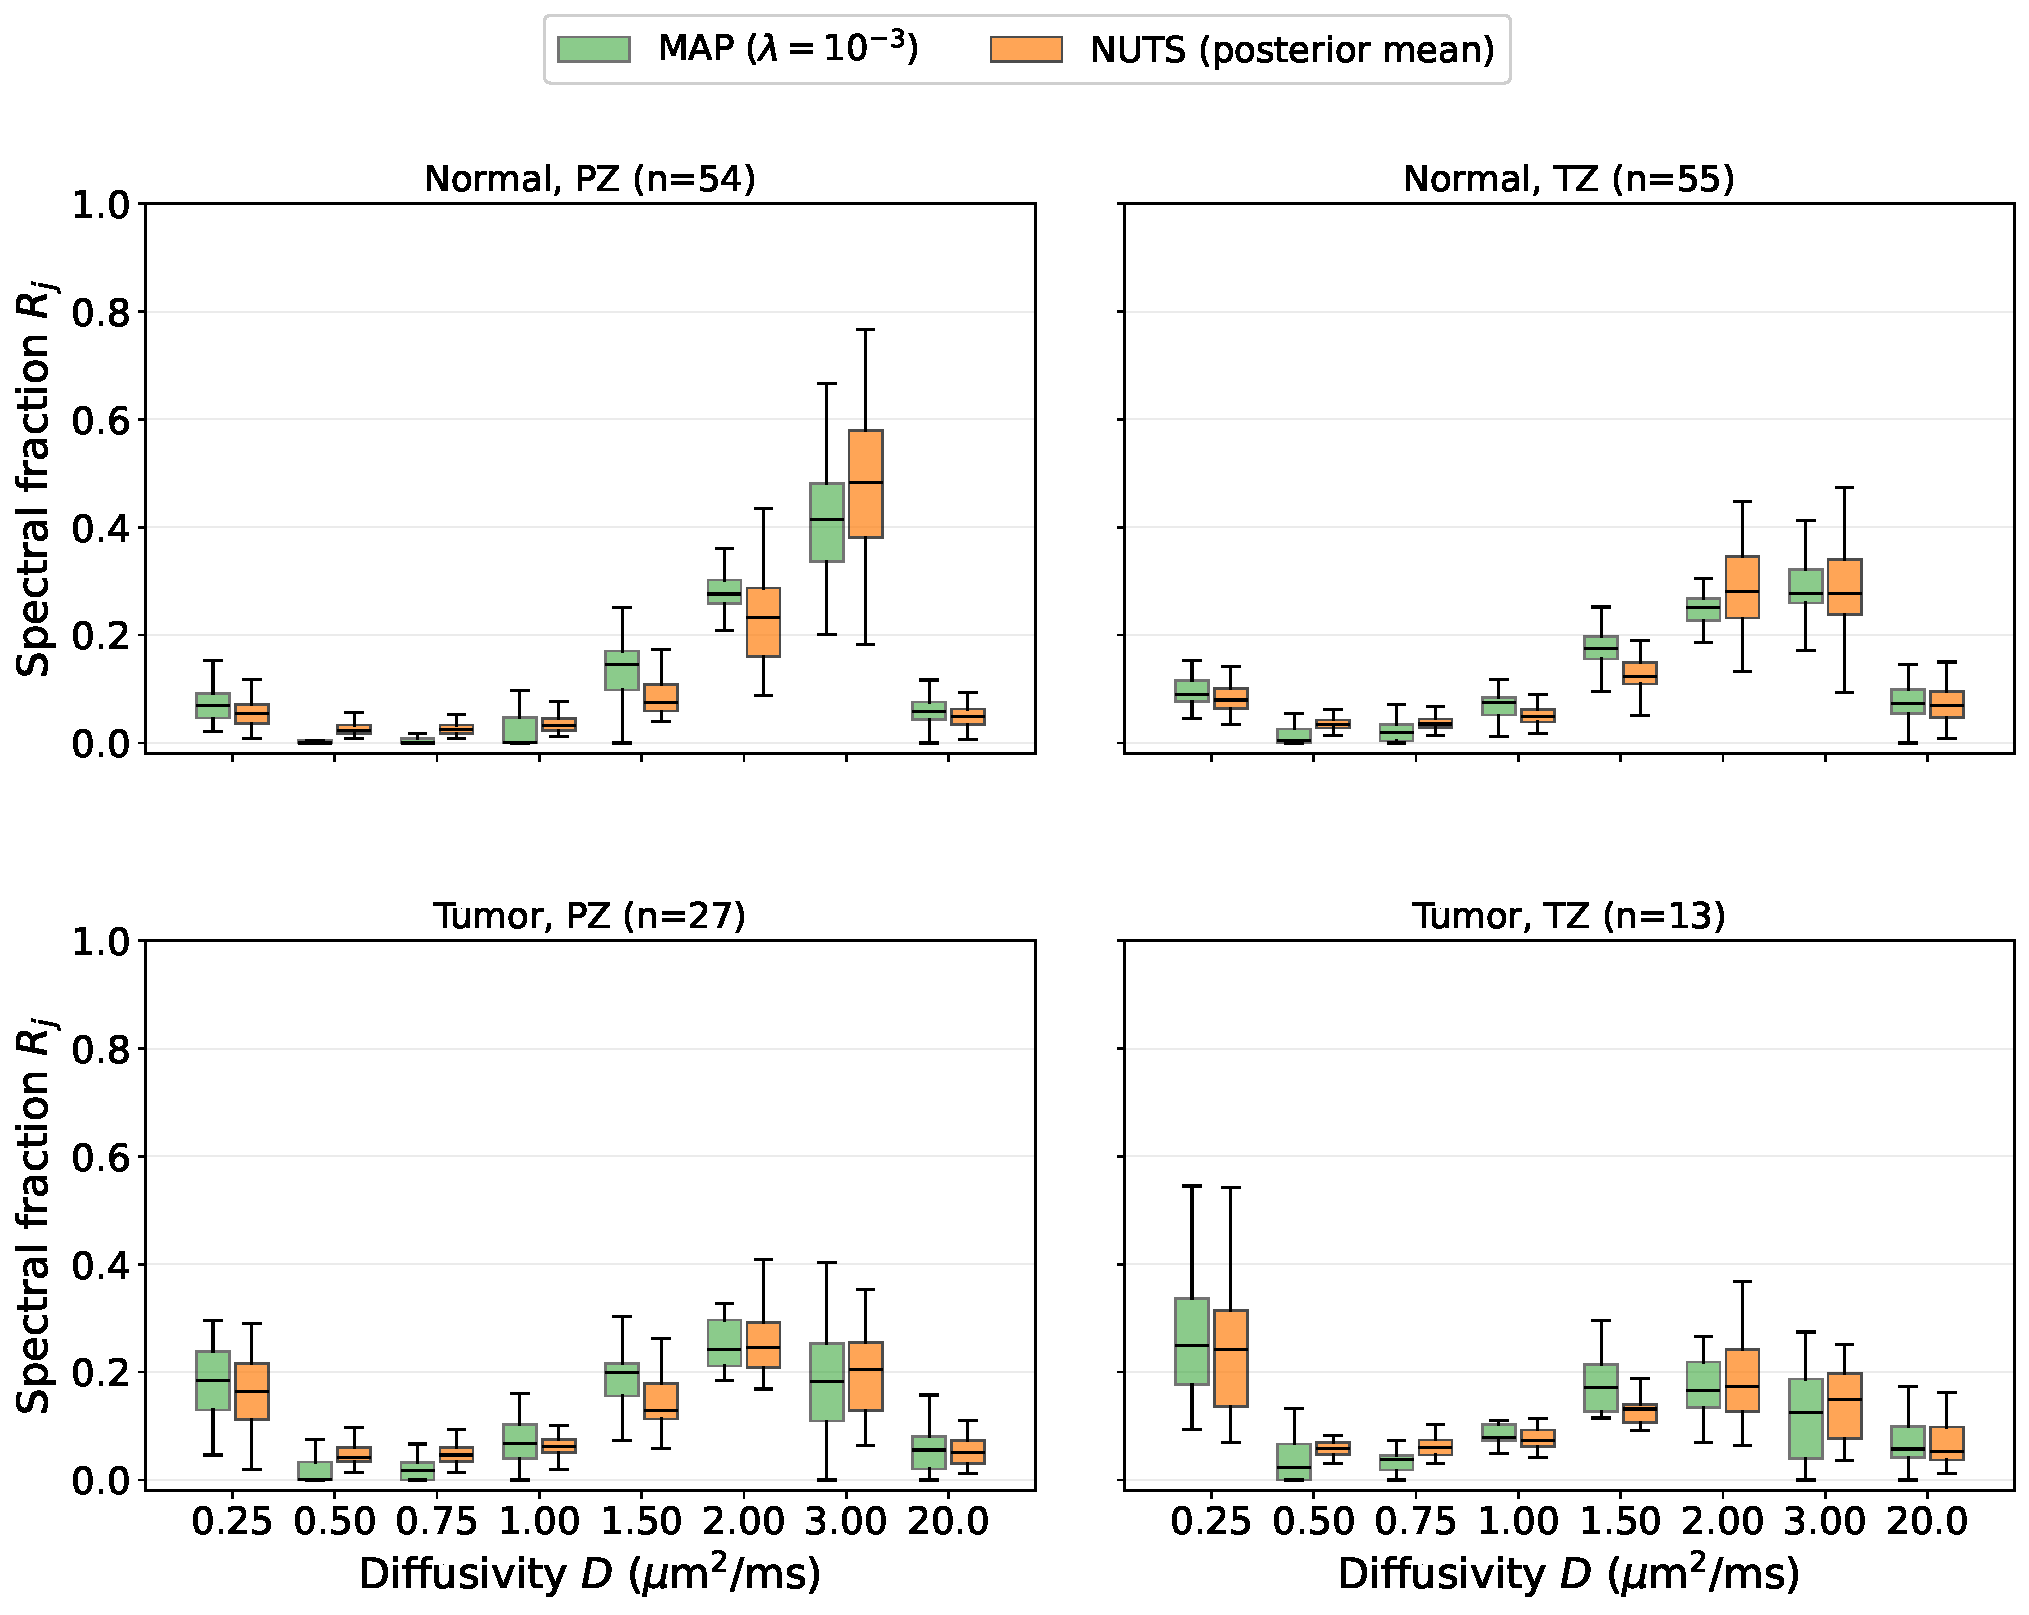
\includegraphics[width=\textwidth]{figures/fig1_v4.pdf}
\caption{%
Cohort diffusivity spectra by tissue type and anatomical zone.
For each diffusivity bin, box plots show the cohort distribution of the
estimated water fraction $R_j$ across ROIs (box: interquartile range; line:
median; whiskers: $1.5\times$ IQR), with MAP (green, hatched) alongside NUTS
posterior-mean estimates (orange) at the tuned regularization
$\lambda = 10^{-3}$.
Top row: normal; bottom row: tumor. Left column: peripheral zone (PZ); right:
transition zone (TZ).
Relative to normal tissue, tumor shows an elevated restricted-diffusion
fraction ($D = 0.25\;\umsmm$) and a reduced free-water fraction
($D = 3.0\;\umsmm$) in both zones, and MAP and NUTS agree closely.
Each box is the cohort distribution of the per-ROI posterior-mean fraction
(between-ROI spread); within-ROI posterior uncertainty is shown in
Figure~\ref{fig:sensitivity} and the supplementary atlas.
}
\label{fig:spectra}
\end{figure}

% --- Fig 2: Tumor-detection ROC; collapse onto the two outer compartments ---
\begin{figure}[p]
\centering
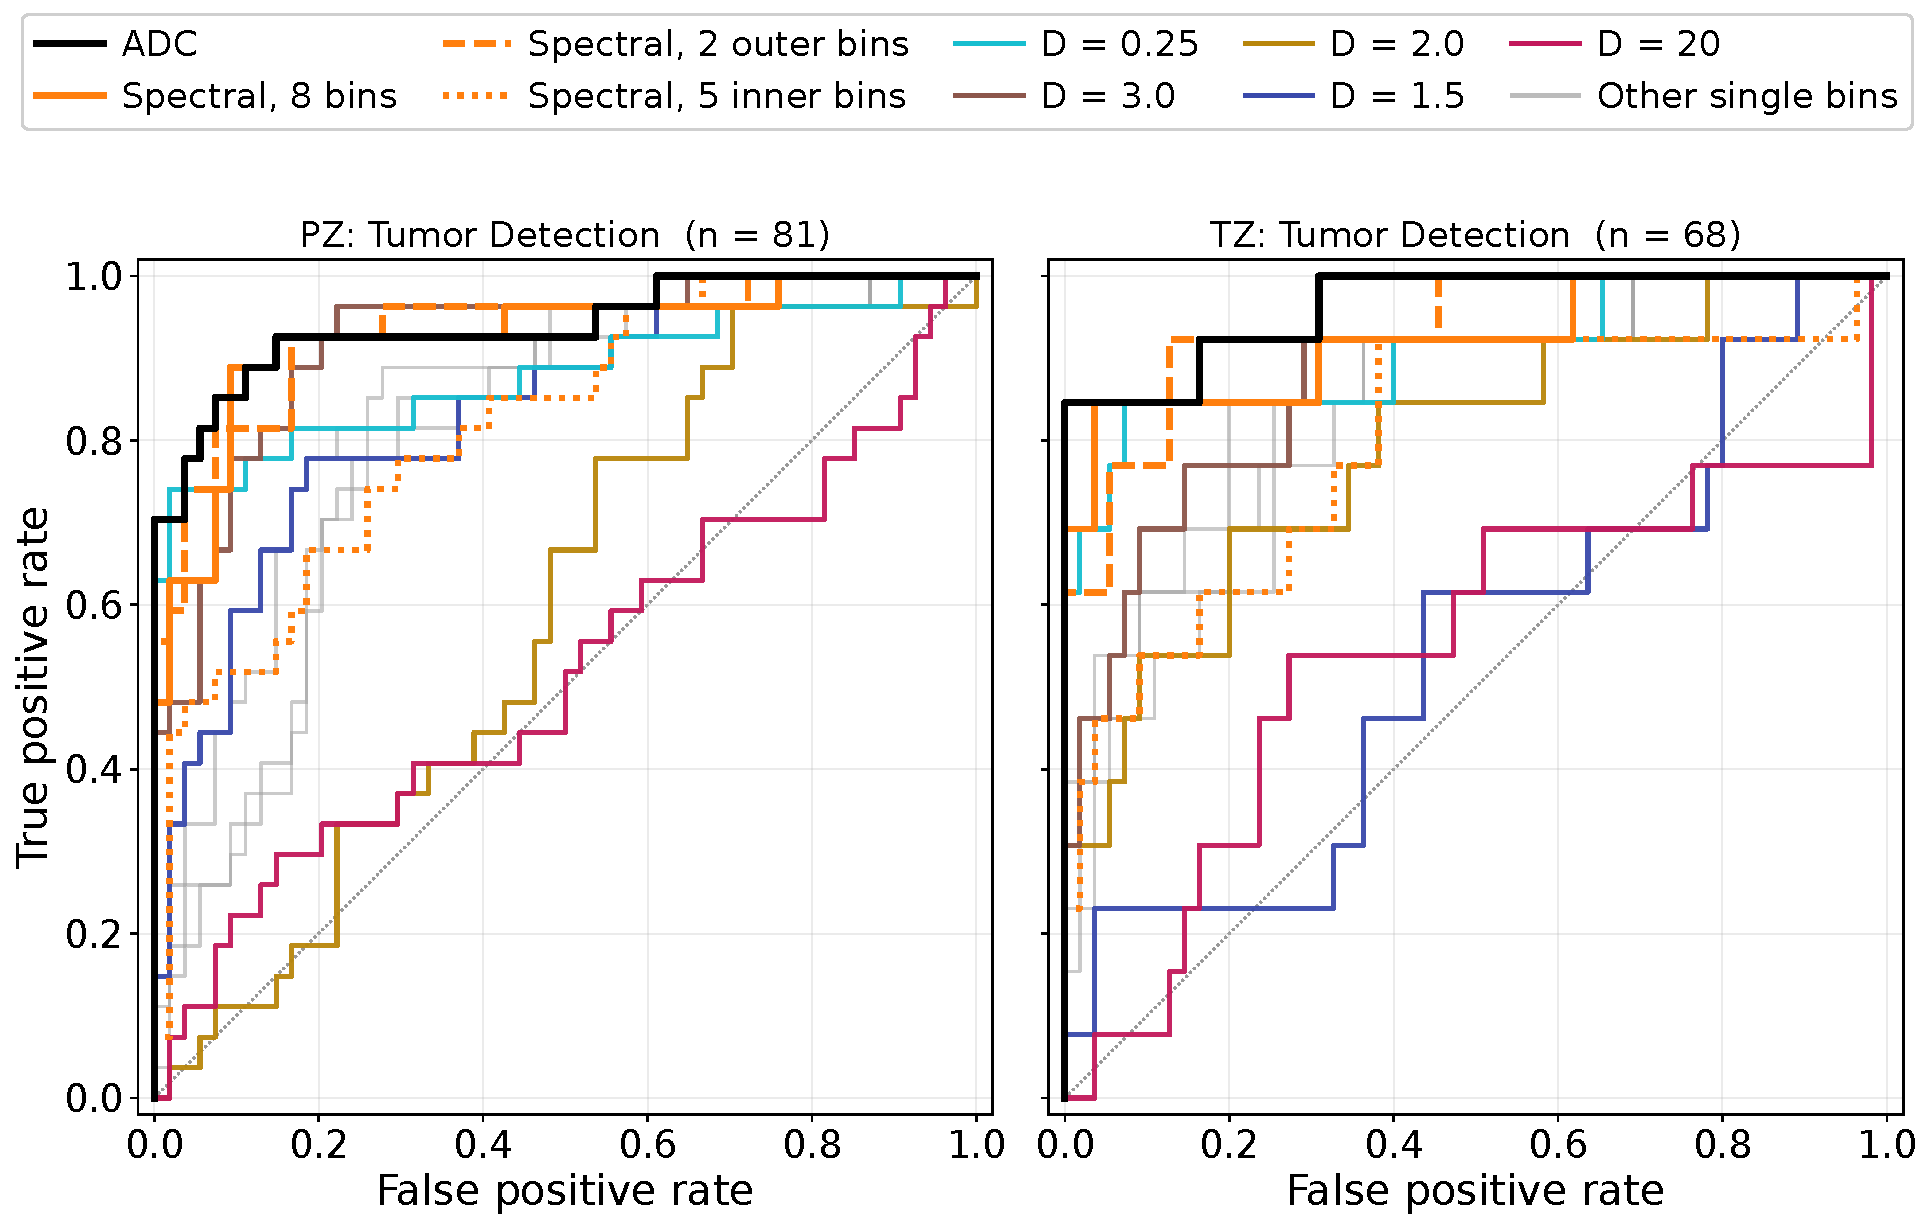
\includegraphics[width=\textwidth]{figures/fig2_v3.pdf}
\caption{%
Tumor detection collapses onto the two outer diffusivity compartments, and the
spectral classifier is equivalent to ADC.
Leave-one-out cross-validated ROC for tumor-versus-normal detection in the
peripheral zone (PZ, left; $n = 81$) and transition zone (TZ, right;
$n = 68$). The three thick reference curves---ADC (black), the spectral
classifier on all eight fractions (orange solid) and on only the two outer
fractions $\{D = 0.25,\,3.0\;\umsmm\}$ (orange dashed)---pass through the
identical NUTS-feature leave-one-out logistic-regression pipeline ($C = 1.0$)
for an apples-to-apples comparison.
The thin single-component curves are each a raw single-feature ROC in the
tumor-positive orientation (not the LOOCV pipeline): the strong outer
components $D = 0.25\;\umsmm$ (restricted, teal) and $D = 3.0\;\umsmm$
(free water, brown), the two weakest bins $D = 2.0\;\umsmm$ (goldenrod) and
$D = 20\;\umsmm$ (magenta), which sit near chance and carry essentially no
detection signal, and the remaining intermediate bins as a faint grey bundle.
The three thick curves are statistically indistinguishable and the
two-fraction classifier matches the full eight-fraction one: the intermediate
and free-water fractions add nothing to detection.
AUC values with 95\% confidence intervals are reported in
Table~\ref{tab:auc}.
}
\label{fig:roc}
\end{figure}

% --- Fig 3: ADC vs Spectral Discriminant ---
\begin{figure}[p]
\centering
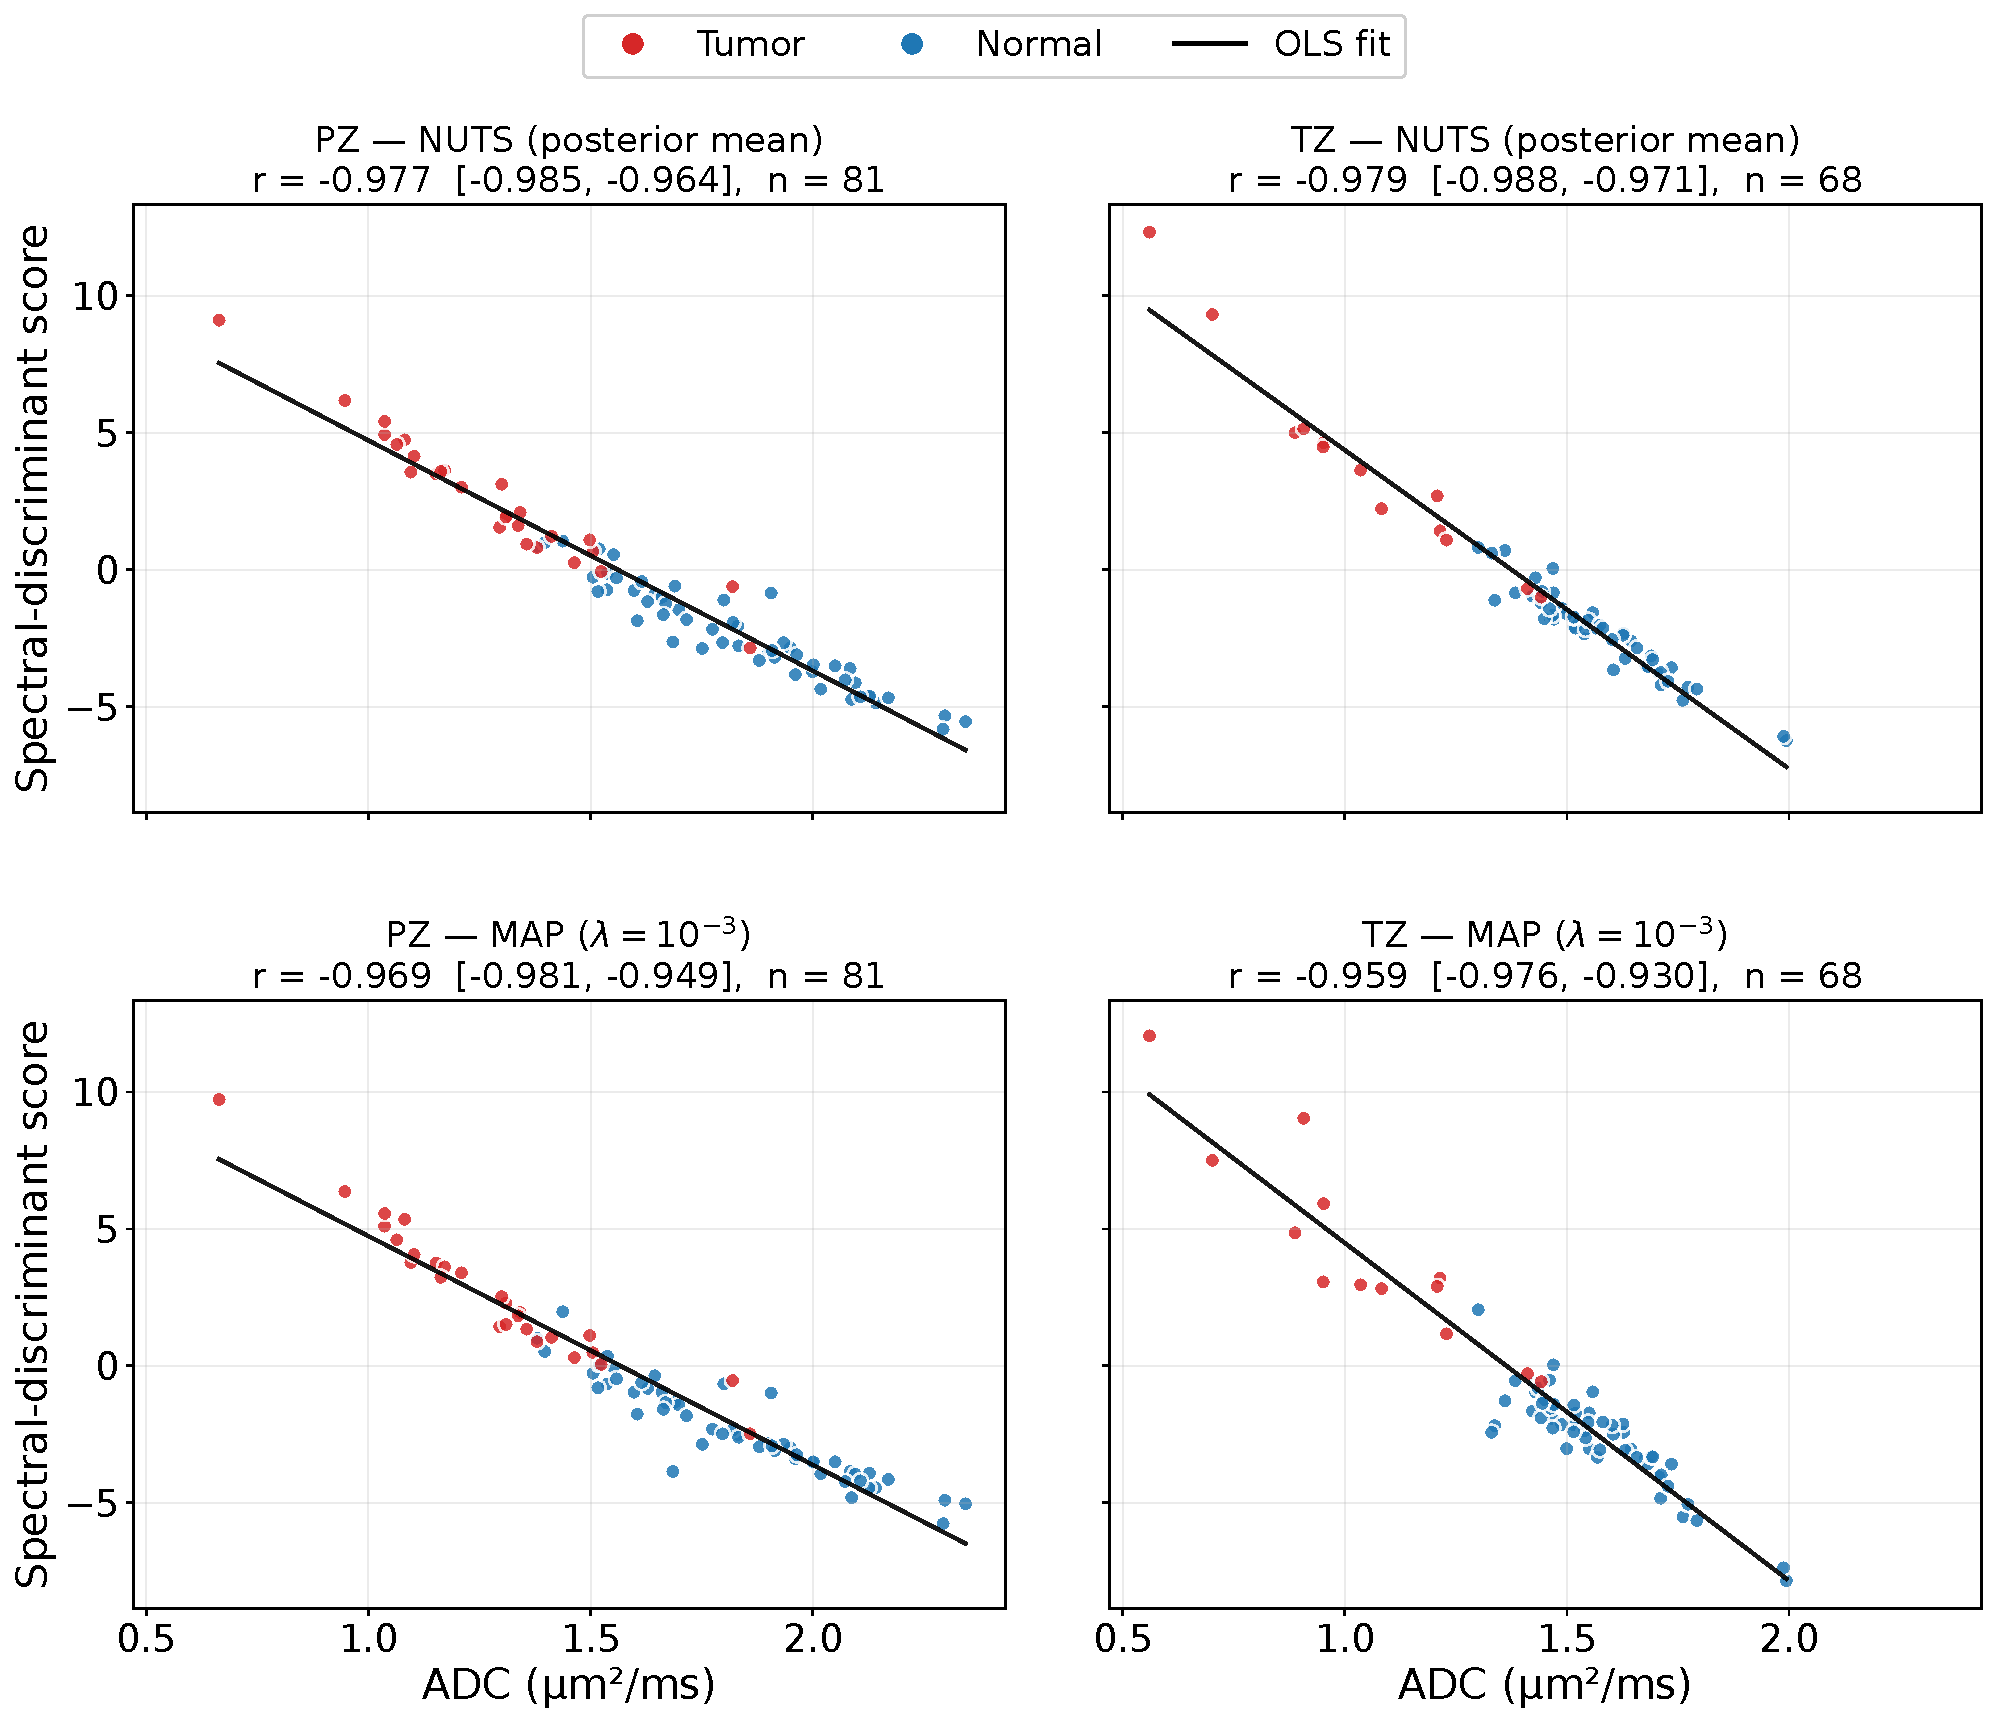
\includegraphics[width=\textwidth]{figures/fig3_v4.pdf}
\caption{%
ADC is a near-optimal spectral discriminant, and the equivalence holds for
both estimators.
ADC versus the spectral discriminant score (logistic-regression linear
predictor from the eight spectral fractions) across ROIs, by anatomical zone
(columns: PZ, $n = 81$, left; TZ, $n = 68$, right) and spectral estimator
(rows: NUTS posterior-mean, top; constrained-MAP at tuned
$\lambda = 10^{-3}$, bottom).
All panels share common axes; the discriminant is fit separately per zone and
estimator, so its score scale is comparable only within a panel, whereas ADC
($x$-axis) is the same physical quantity throughout.
Tumor ROIs (red) cluster at low ADC and high discriminant, normal ROIs (blue)
the reverse; the black line is the OLS fit.
Per-panel Pearson $r$ with a 95\% percentile-bootstrap confidence interval is
annotated in each panel (all $|r| > 0.95$).
The near-perfect anti-correlation shows that ADC rank-orders ROIs almost
identically to the spectral classifier, independent of estimator.
}
\label{fig:adc_discriminant}
\end{figure}

% --- Fig 4: per-bin anatomy of the spectral discriminant ---
\begin{figure}[p]
\centering
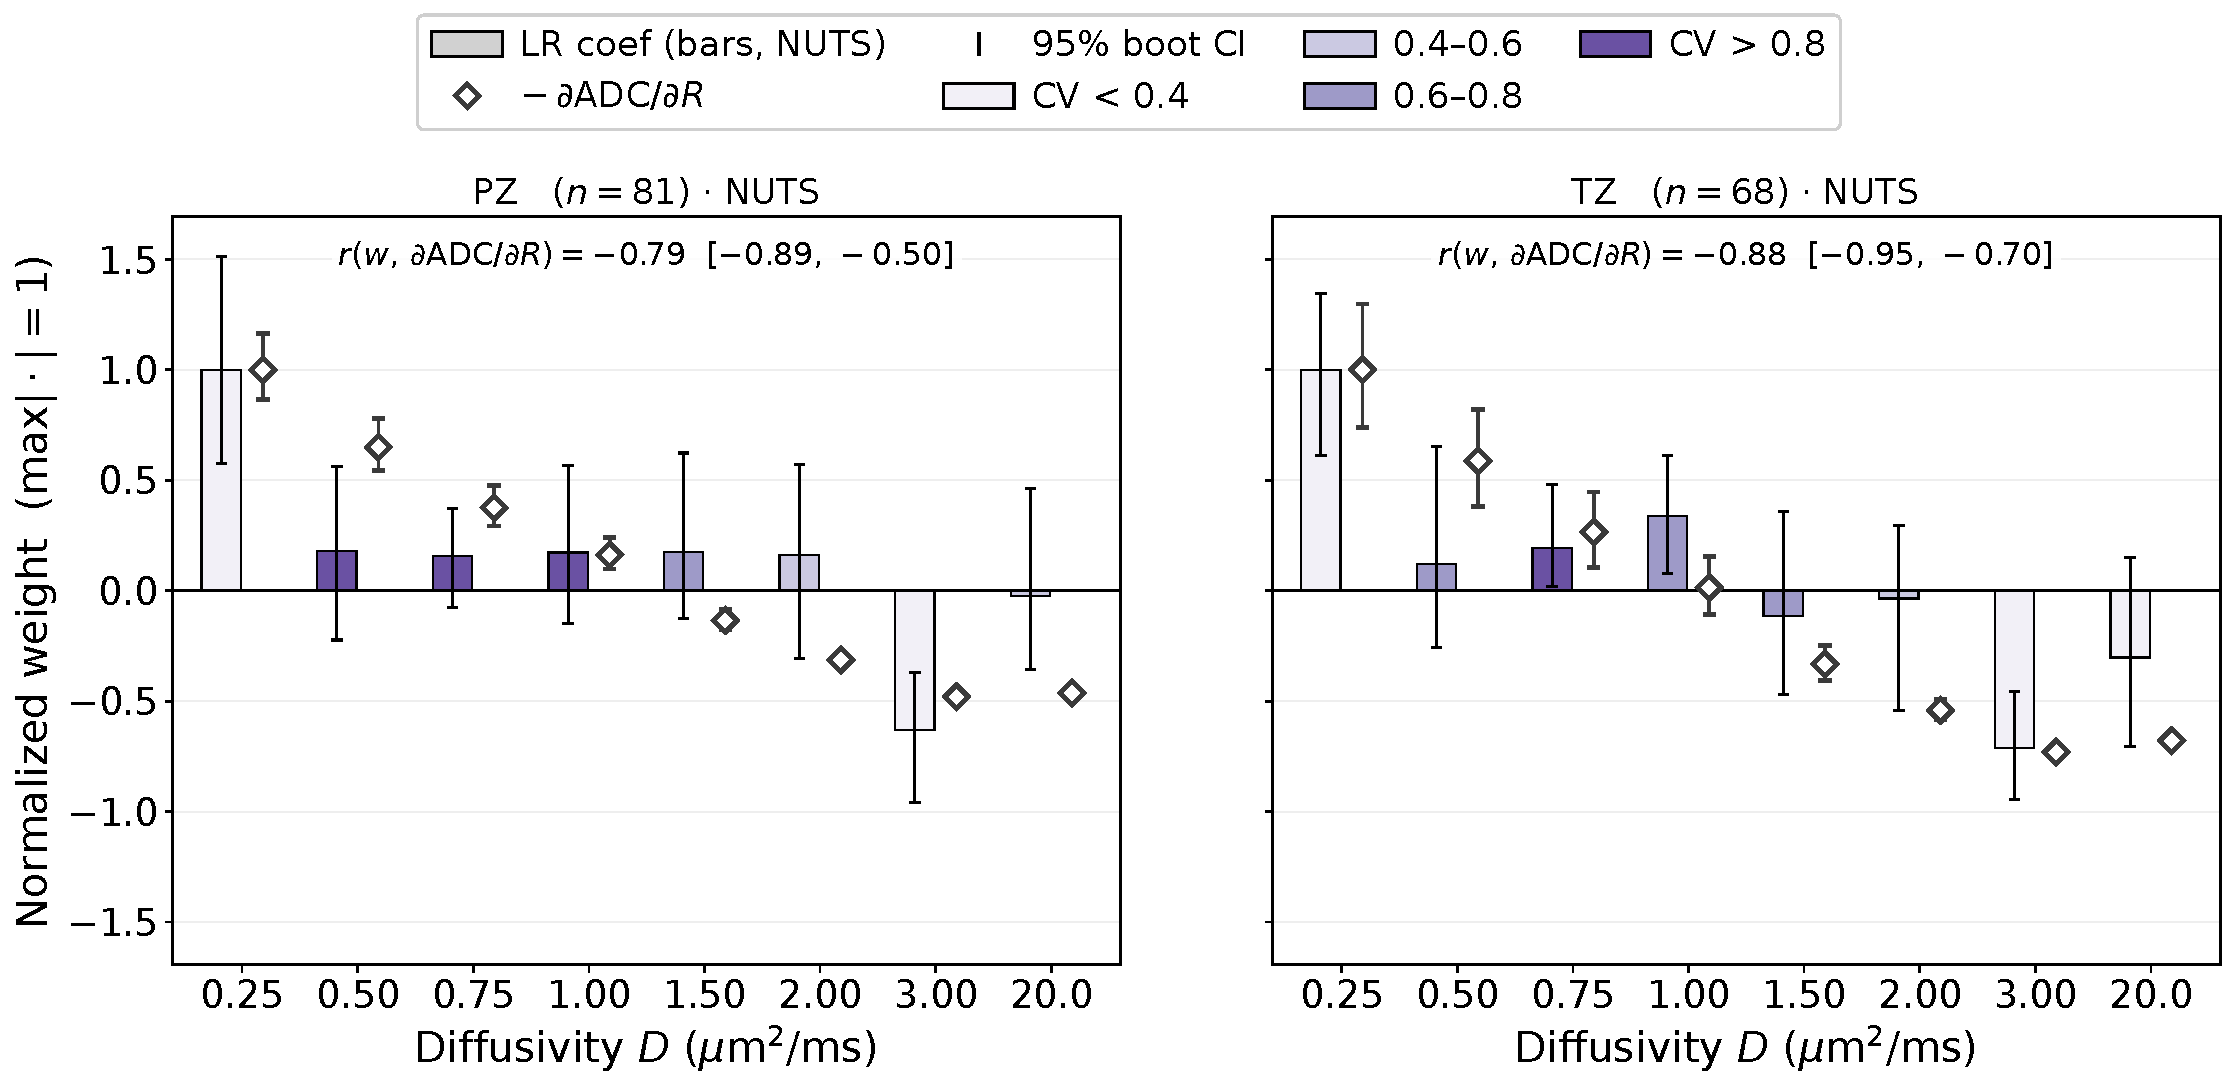
\includegraphics[width=\textwidth]{figures/fig4_std_v4.pdf}
\caption{%
The spectral discriminant is statistically a two-compartment detector, and its
two stable bins coincide with where ADC is most sensitive.
For each zone (PZ, TZ), bars give the standardized tumor-versus-normal
logistic-regression coefficient per diffusivity bin (NUTS features, $C = 1.0$,
the same fit as Figure~\ref{fig:adc_discriminant}), normalized to
$\max|w| = 1$, with 95\% bootstrap confidence intervals.
Charcoal diamonds give the ADC sensitivity $-\partial\text{ADC}/\partial R_j$
at the average tumor spectrum (normalized, sign-aligned to the tumor
direction).
Each bar is colored and hatched by the bin's within-ROI posterior CV (light
$=$ well identified to dark $=$ poorly identified), a per-ROI identifiability
distinct from the cohort-level coefficient stability shown by the bootstrap
intervals.
In both zones only the two outer bins carry stable weight ($D = 0.25\;\umsmm$
positive, $D = 3.0\;\umsmm$ negative); the intermediate coefficients are
individually unstable from inter-bin collinearity and poor identifiability, so
their separate detection weights are not attributable.
The profile anti-correlates with $\partial\text{ADC}/\partial R_j$
($r = -0.79$ PZ, $-0.88$ TZ), carried by the two outer bins---weaker than the
near-unity value seen under heavy regularization ($\lambda = 0.1$), where
smearing artificially smooths the profile (see Discussion).
The intermediate bins' value appears instead as a grading signal
(Figure~\ref{fig:spectrum_ggg}).
}
\label{fig:sensitivity}
\end{figure}

% --- Fig 5: Diffusivity Spectrum by Gleason Grade Group (single-panel ladder) ---
\begin{figure}[p]
\centering
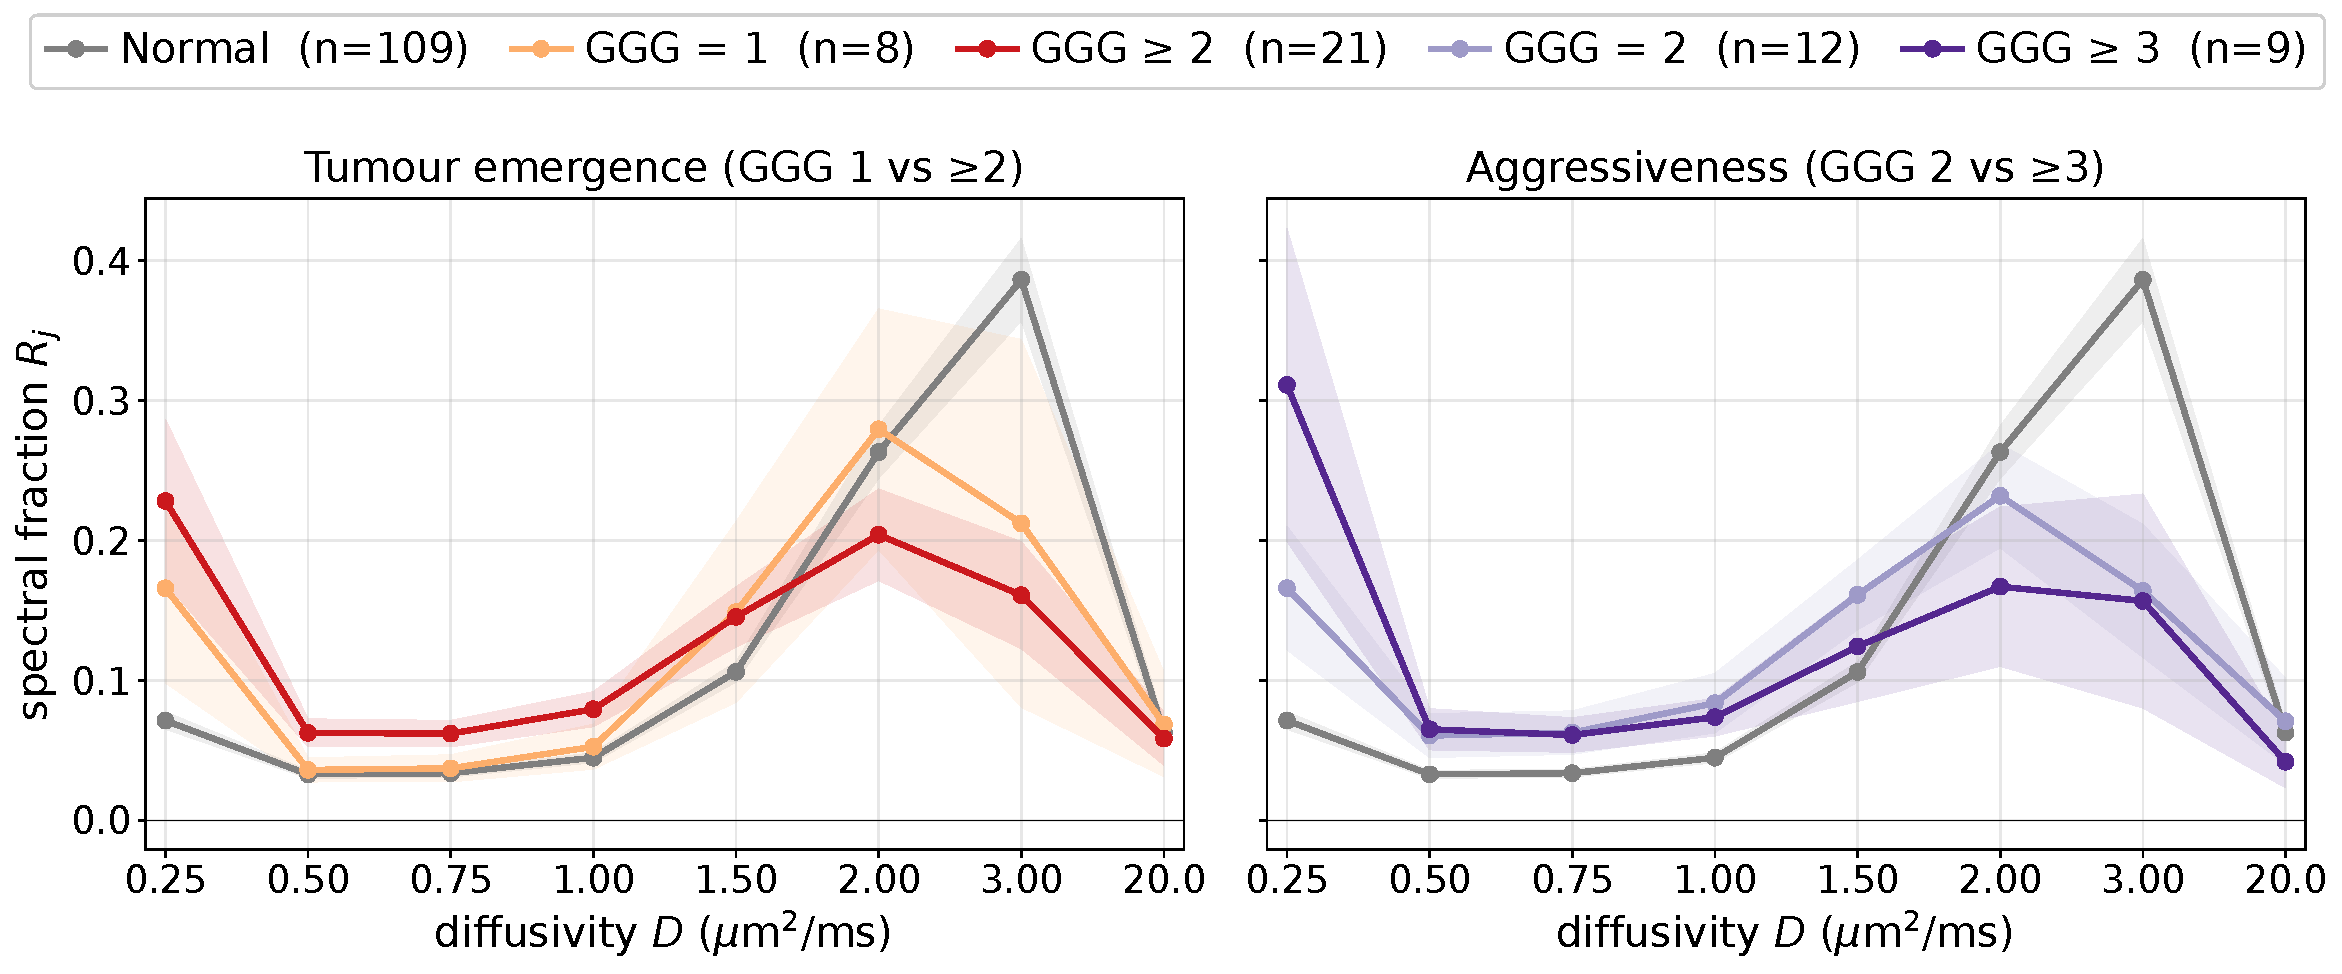
\includegraphics[width=\textwidth]{figures/fig5_v5.pdf}
\caption{%
The diffusivity spectrum by Gleason Grade Group reveals a detection axis
distinct from a grading axis.
NUTS posterior-mean spectrum averaged across ROIs, in two contrasts that share
a normal-tissue baseline (gray, $n = 109$). Left (emergence): GGG\,$=\,1$
($n = 8$) versus GGG\,$\geq 2$ ($n = 21$). Right (aggressiveness): GGG\,$=\,2$
($n = 12$) versus GGG\,$\geq 3$ ($n = 9$). Each grade group has its own color.
Shaded bands are 95\% confidence intervals of the group mean (Student's $t$,
$\text{df} = n - 1$).
The free-water bin ($D = 3.0\;\umsmm$, a proxy for intact gland lumen)
collapses at tumor onset ($0.39$ normal $\to 0.21$ at GGG\,$=\,1$) and changes
little thereafter ($0.16$ at GGG\,$\geq 3$): it carries detection, not grade.
In contrast the restricted-cellular bin ($D = 0.25\;\umsmm$) and the
glandular-epithelial bin ($D = 2.0\;\umsmm$), where ADC is least sensitive,
track grade: $D = 0.25$ rises with grade ($0.07$ normal, $0.17$ at
GGG\,$=\,1$--$2$, $0.31$ at GGG\,$\geq 3$) and $D = 2.0$ is preserved in
low-grade tumor then depleted ($0.26$ normal, $0.28$ at GGG\,$=\,1$, $0.17$ at
GGG\,$\geq 3$).
Grade groups are small (down to $n = 8$--$9$) and the bands wide; 11 of 40
tumor ROIs (7 with GGG\,$=\,0$, 4 ungraded) are not shown.
}
\label{fig:spectrum_ggg}
\end{figure}

% --- Fig 6: Uncertainty-aware classifier (posterior propagation) ---
\begin{figure}[p]
\centering
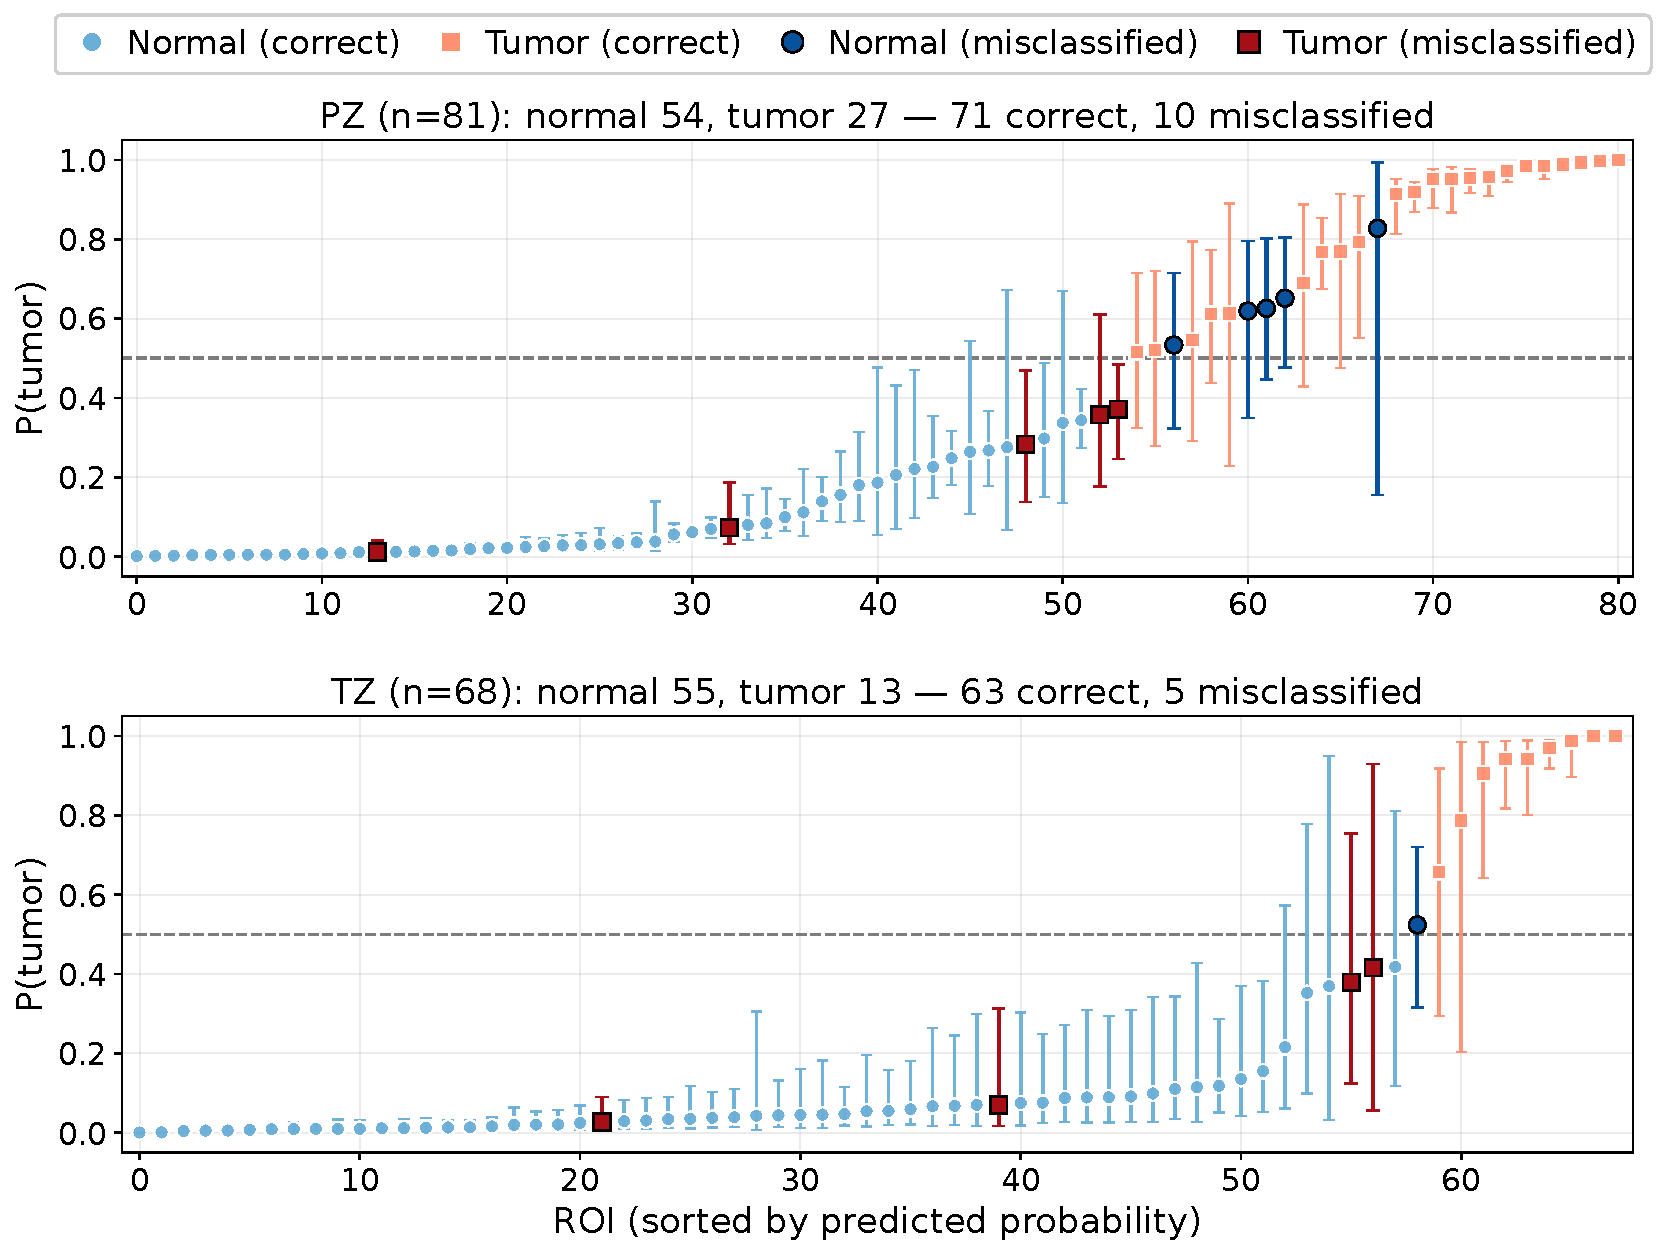
\includegraphics[width=\textwidth]{figures/fig6_v2.pdf}
\caption{%
Propagating the diffusivity-spectrum posterior through the classifier turns a
binary label into a calibrated probability of cancer whose uncertainty is
largest where the classifier is most likely to be wrong.
For each ROI the leave-one-out classifier (the same NUTS-feature pipeline as
Figure~\ref{fig:roc}, $C = 1$) is applied to every NUTS posterior draw of the
eight fractions, yielding a posterior distribution over $P(\mathrm{tumor})$
rather than a point estimate.
Per-ROI predictions in the peripheral zone (top, $n = 81$) and transition zone
(bottom, $n = 68$), each ROI sorted by its predicted probability: markers at
the posterior-mean probability (circles normal, squares tumor) with error bars
the propagated 90\% credible interval; correctly classified ROIs are shown in
pale colors and misclassified ROIs in saturated colors.
Two uncertainties are evident. First, the credible interval is on average
$2.4\times$ wider for misclassified than for correctly classified ROIs (pooled
mean width $0.39$ vs $0.16$; Welch $p = 0.003$). Second, intervals widen toward
the decision boundary ($P = 0.5$); this widening is partly a geometric property
of the logistic link---in logit space both the boundary effect and the
misclassified-to-correct width ratio shrink markedly---but a genuine residual
remains.
The residual confidently-misclassified ROIs are almost all low-grade or
ungraded tumors whose spectra resemble normal tissue
(cf.\ Figure~\ref{fig:spectrum_ggg})---a limit of diffusion contrast, not a
failure of the uncertainty estimate.
A MAP point estimate cannot produce these intervals.
This analysis is exploratory.
}
\label{fig:uncertainty}
\end{figure}

% --- Fig 7: Direction independence (whole-ROI) ---
% Generator: scripts/fig7_directions_roi.py (decodes the per-direction ROI .dat
% export; MAP spectra via recompute.compute_map_spectrum). Patient 9283, the
% only matched same-zone (PZ) normal+tumour pair. Aggregate per-direction CV
% over all 13 ROIs is reported in Results.
\begin{figure}[p]
\centering
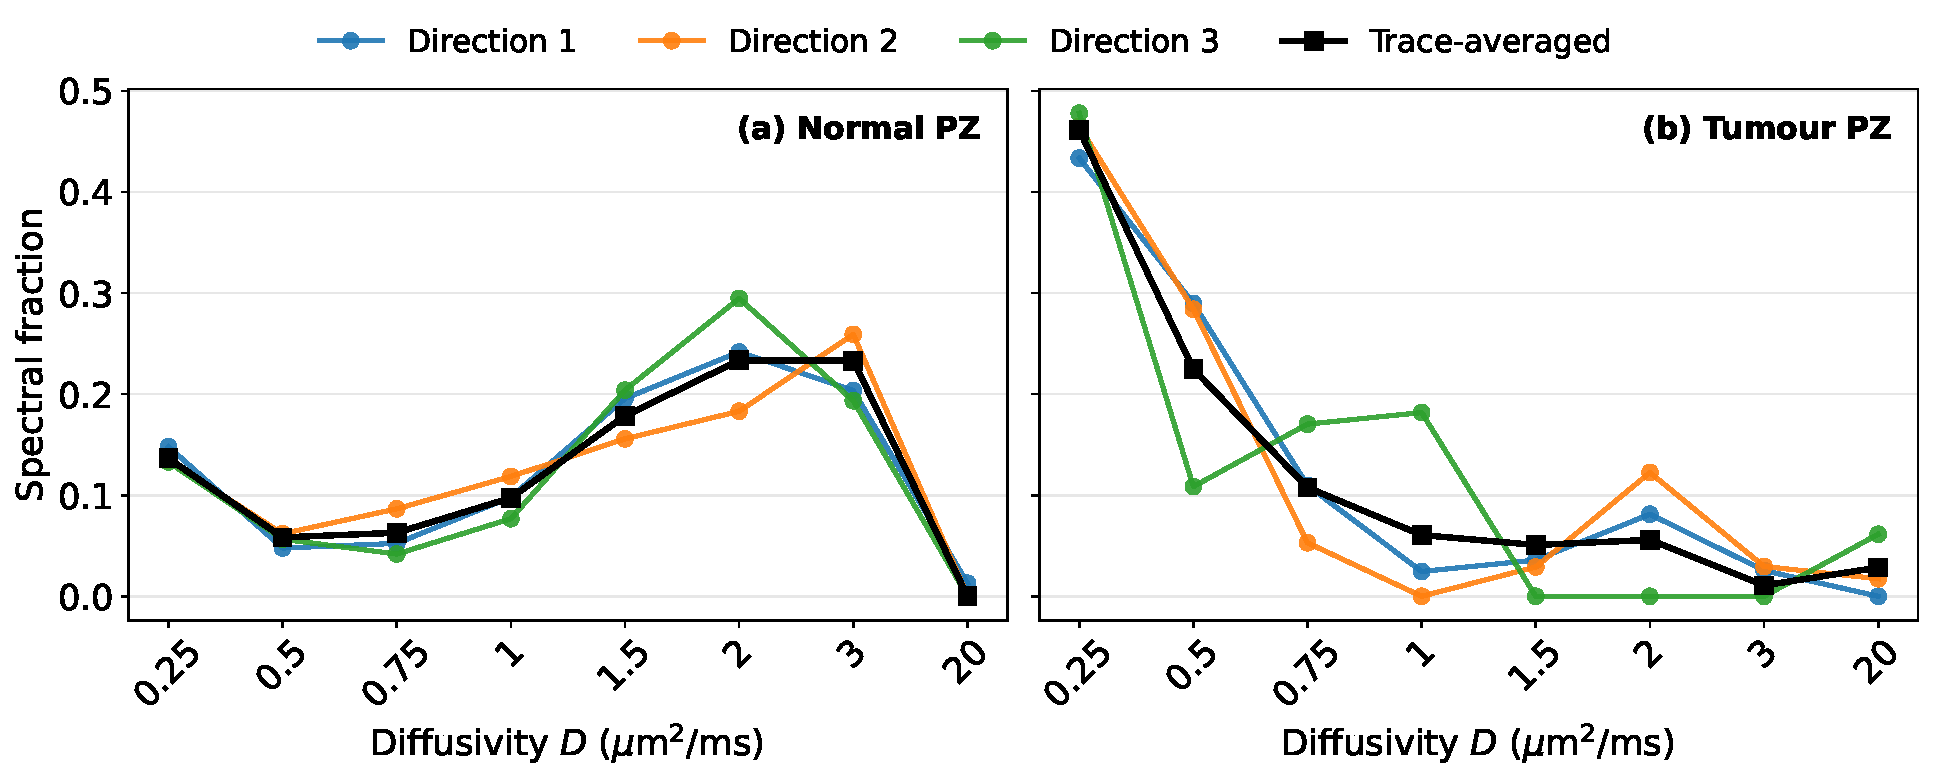
\includegraphics[width=\textwidth]{figures/fig_directions_v2.pdf}
\caption{%
Direction independence of whole-ROI spectral estimates validates trace
averaging.
Per-encoding-direction MAP spectra (three encoding directions) versus the
trace-averaged spectrum (black) for (a)~a normal and (b)~a tumor
peripheral-zone region of interest in a representative patient.
The three directions agree closely in the diagnostically dominant
restricted-diffusion bin ($D = 0.25\;\umsmm$; mean direction-wise CV $9\%$
across all 13 regions); the larger inter-direction spread in the intermediate
and near-empty bins ($D = 0.5$--$2.0$ and $D = 20\;\umsmm$) mirrors their poor
identifiability rather than reflecting genuine anisotropy, the per-direction
CV tracking each bin's inverse mass.
Because tumor detection rests on the well-identified outer compartments, trace
averaging is well justified; aggregate per-bin statistics are reported in
Results.
MAP estimates are shown (constrained ridge, $\lambda = 10^{-3}$); MAP and NUTS
are equivalent on realistic spectra (Figure~\ref{fig:validation}).
}
\label{fig:directions}
\end{figure}

% --- Fig 8: Method validation on simulated ground truth (spectrum x SNR battery) ---
% Generator: scripts/fig8_battery.py (replots from cached
% results/simulation/fig8_battery_snr.npz; --regen resamples). 4 ground truths
% x 2 SNR recovery grid + joint-noise sigma-calibration panel. No Gibbs
% (deferred). Real pipeline: nuts.yaml + tuned-MAP ridge.yaml.
\begin{figure}[p]
\centering
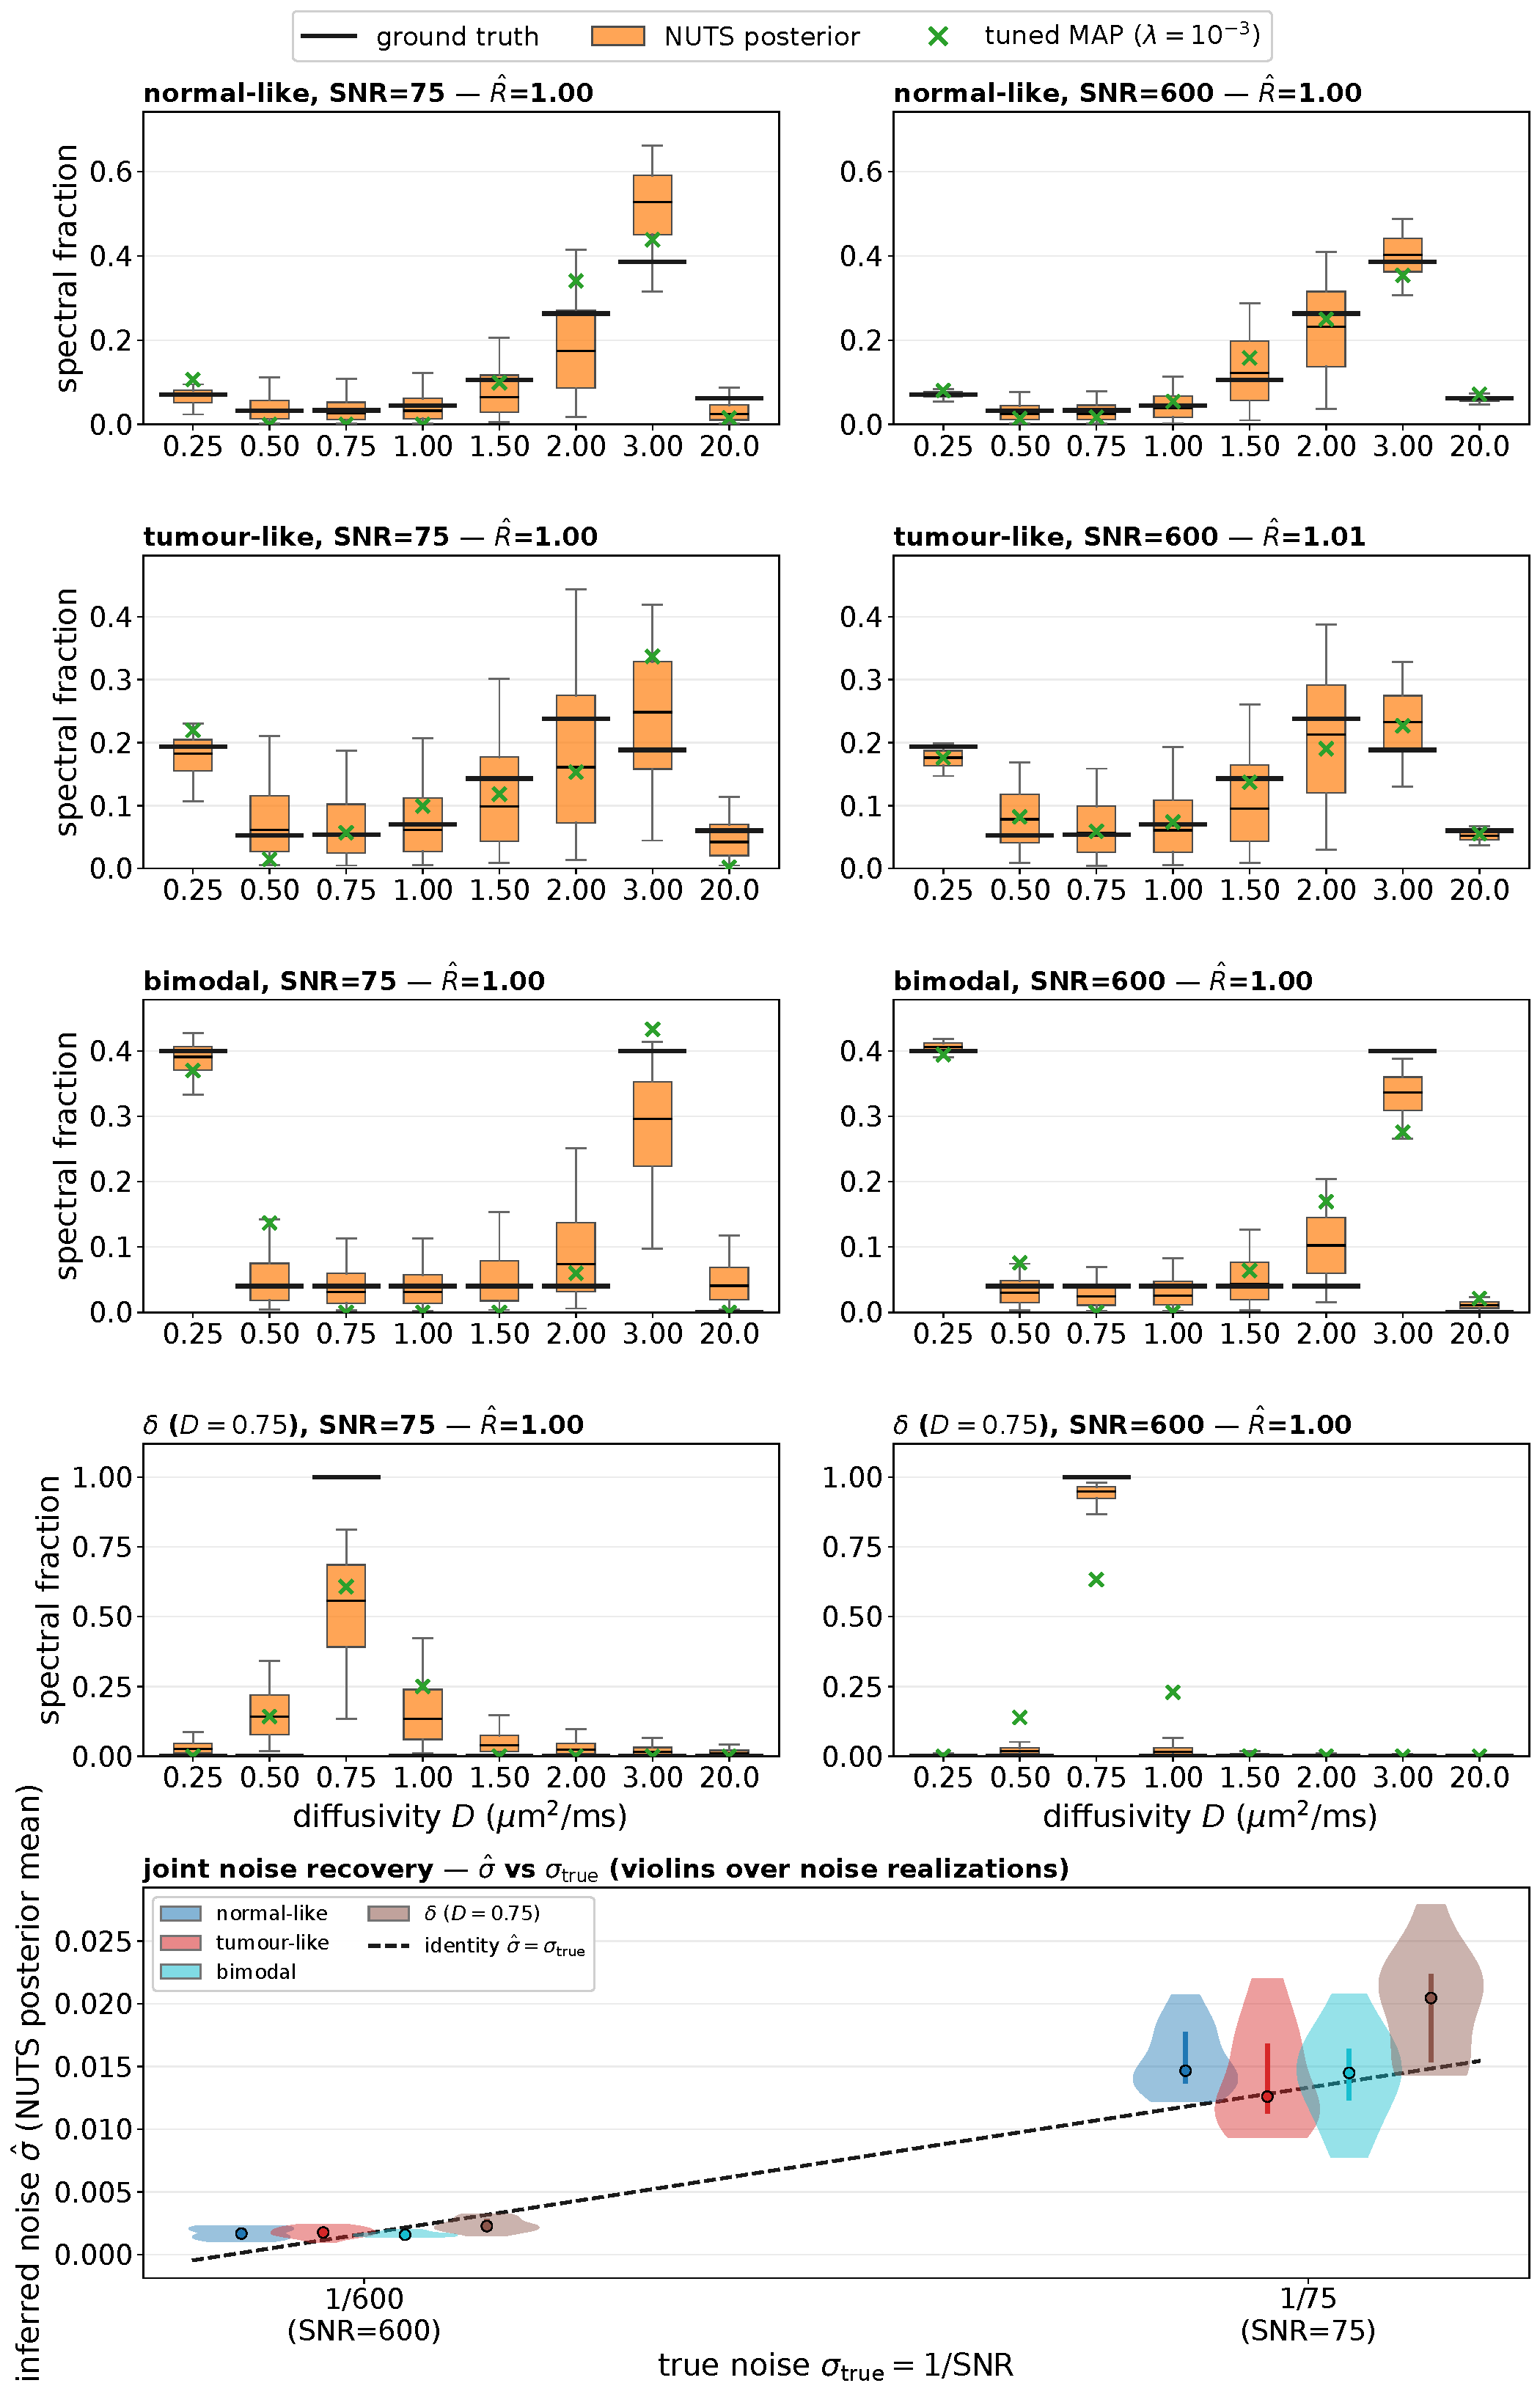
\includegraphics[width=\textwidth]{figures/fig8_v5.pdf}
\caption{%
Validation of the Bayesian spectral inference on simulated ground truth across
spectrum shape and signal-to-noise ratio.
Four ground-truth spectra---a normal-like and a tumor-like spectrum (the
cohort-mean NUTS spectra), a bimodal spectrum (mass at $D = 0.25$ and
$3.0\;\umsmm$), and a concentrated $\delta$ at $D = 0.75\;\umsmm$---are each
recovered at a low (SNR $= 75$) and a high (SNR $= 600$) noise level that
bracket the cohort median (303).
In each panel the black marks are the truth, the orange box plots the NUTS
posterior for one noisy realization (box $=$ interquartile range, whiskers
$=$ 5th--95th percentile), and the green cross the tuned-MAP estimate
($\lambda = 10^{-3}$); the split-$\hat{R}$ convergence diagnostic is reported
in each panel title (all $\hat{R} \leq 1.01$).
The smooth spectra are recovered well at both SNRs (tighter at high SNR),
whereas the $\delta$ spike is under-recovered and smeared into its correlated
neighboring bins---the genuine identifiability limit of this b-value grid, not
a sampler artifact.
The bottom panel shows joint noise inference: the inferred noise
$\hat{\sigma}$ (NUTS posterior mean over 12 realizations per condition, drawn
as violins) versus the true $\sigma = 1/\mathrm{SNR}$ (dashed identity line).
$\sigma$ is recovered to within $\sim$10\% for the smooth spectra but is
over-estimated by $\sim$35--50\% on the $\delta$, where the model absorbs the
unrepresentable spike as excess noise (consistent with the coverage caveat
discussed below).
}
\label{fig:validation}
\end{figure}

% --- Fisher Information Analysis: lives in the Supplement (sections/supporting.tex) ---
% The \label{fig:fisher} is defined there, so the in-text references in
% theory/results/discussion resolve to a supplementary figure.

% --- Fig 9: Pixel-wise Spectral Decomposition ---
\begin{figure}[p]
\centering
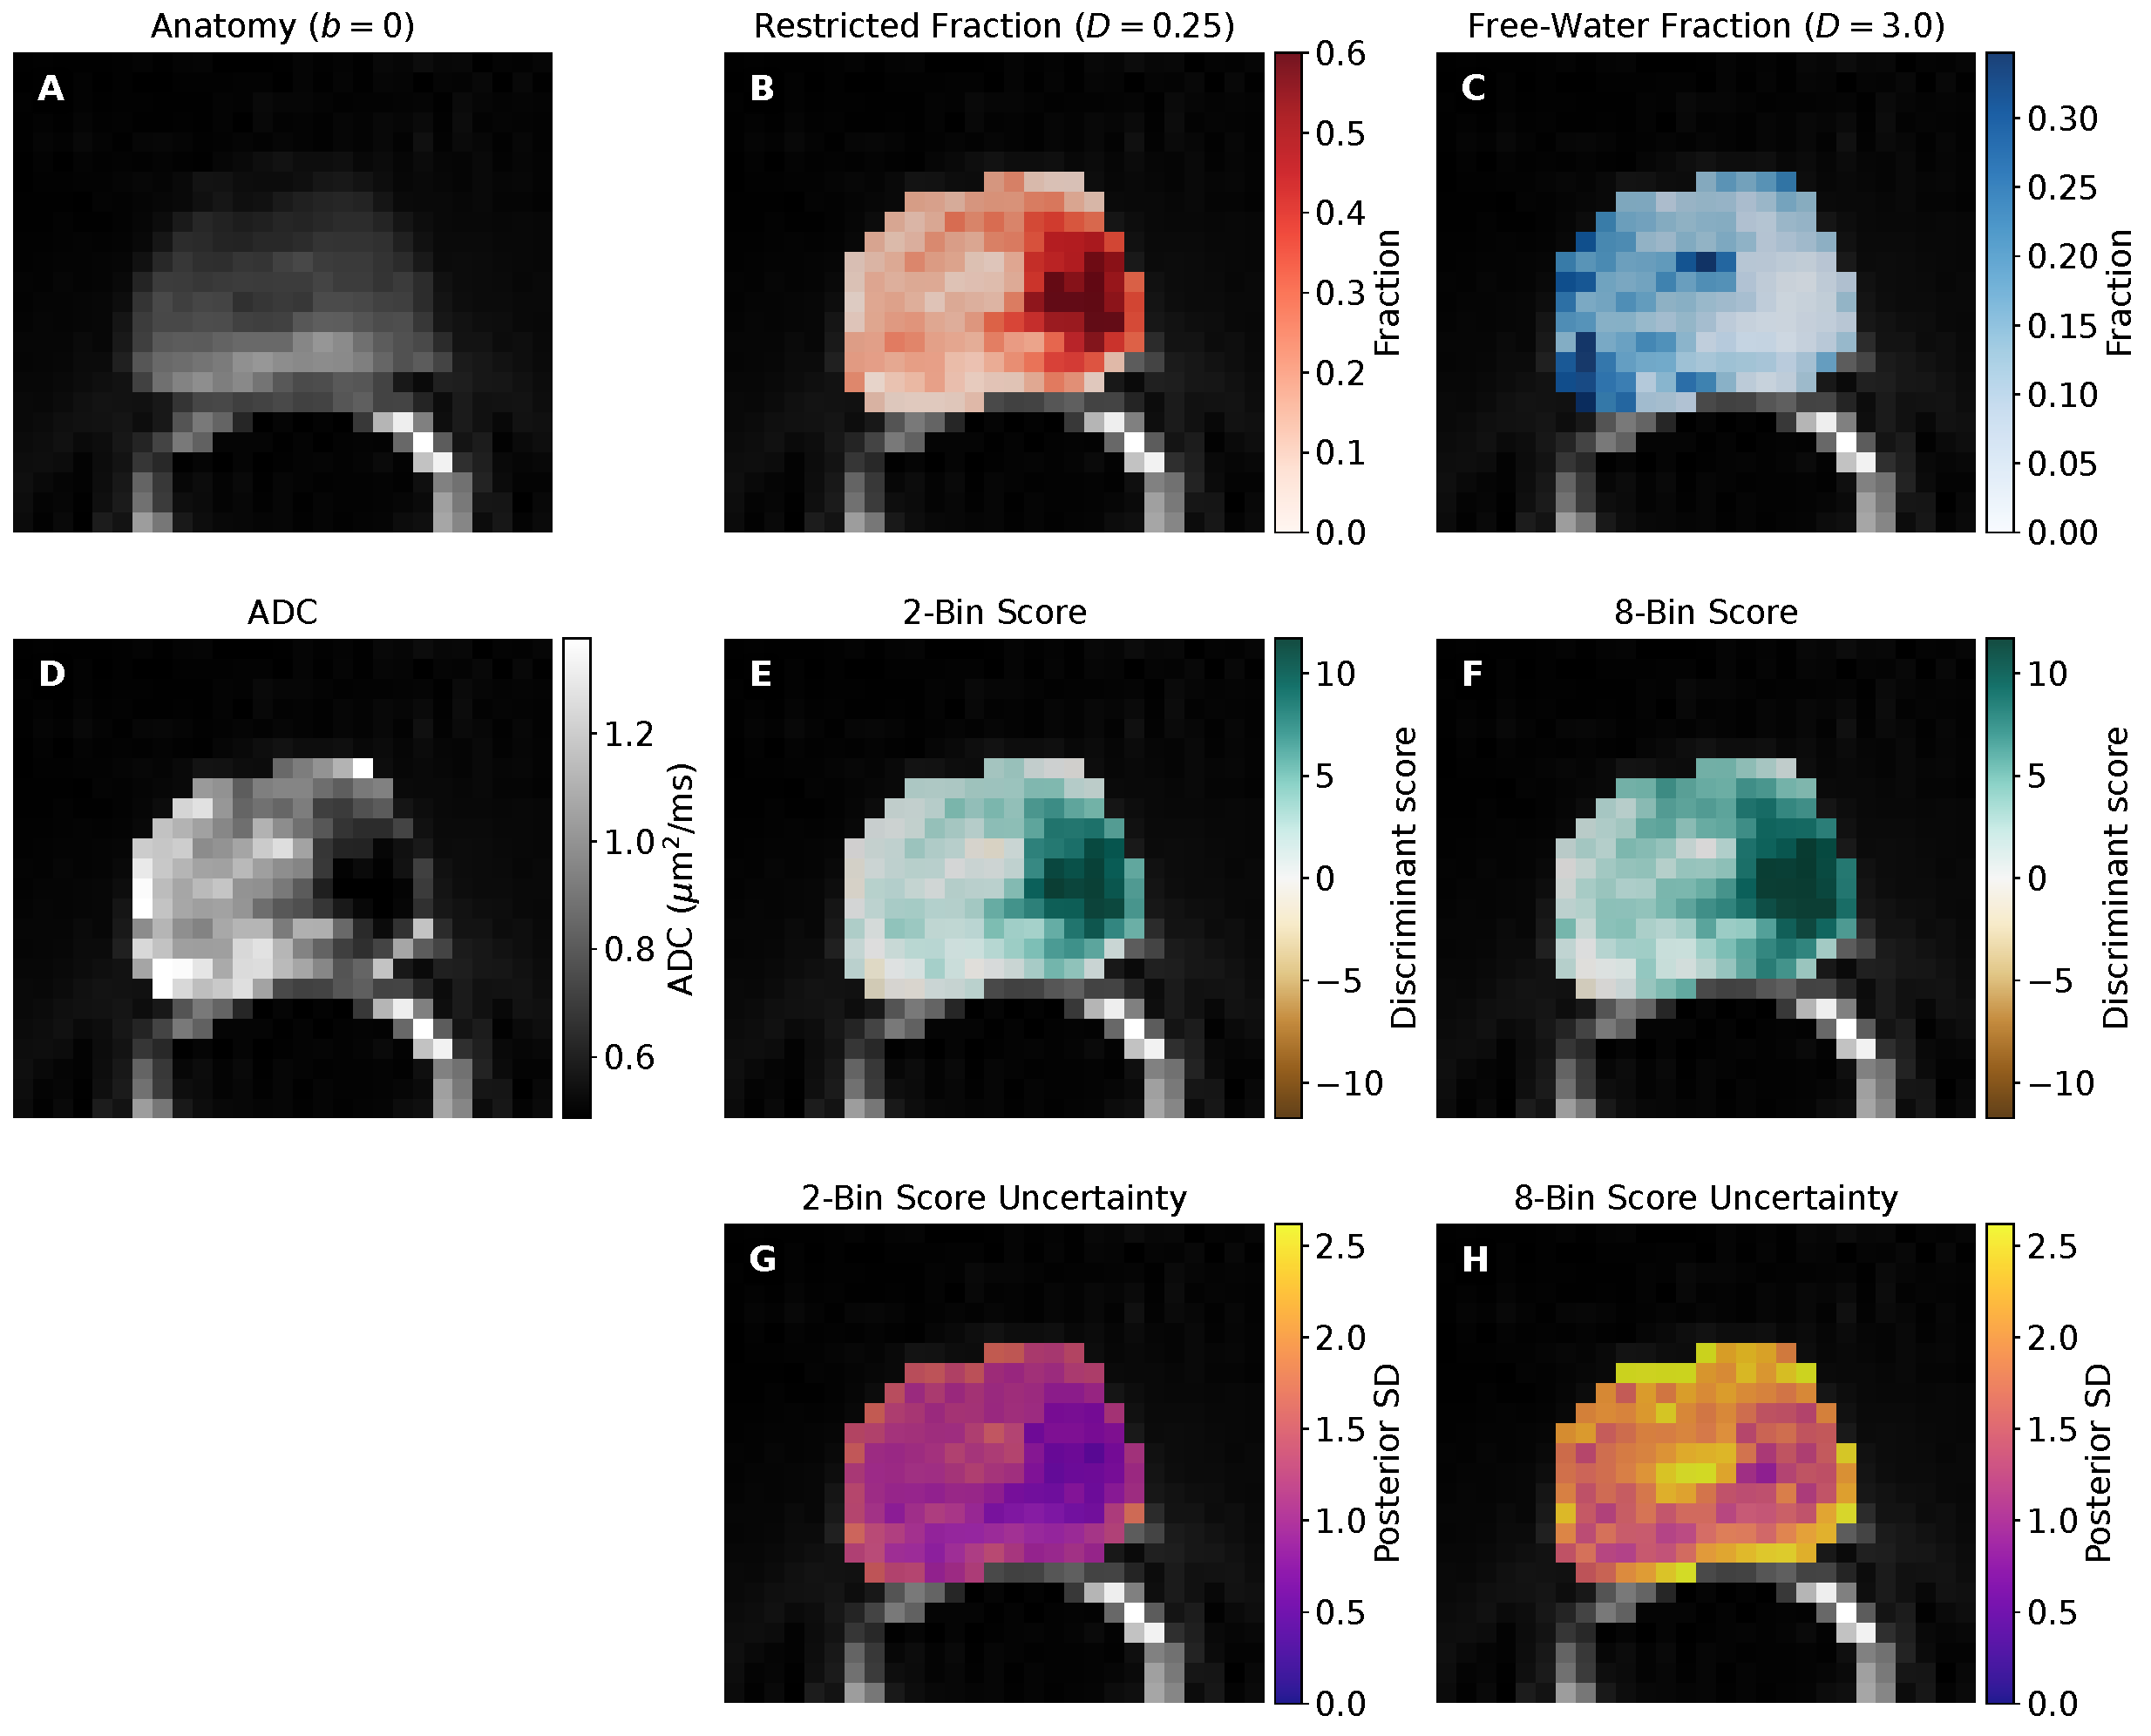
\includegraphics[width=\textwidth]{figures/fig9_v2.pdf}
\caption{%
Pixel-wise spectral decomposition of a single peripheral-zone prostate DWI
slice (anonymized patient), showing that the ROI-level detector extends to the
voxel level while uniquely providing a per-voxel uncertainty map.
(A)~Anatomical reference ($b = 0$).
(B,\,C)~NUTS posterior-mean restricted-diffusion ($D = 0.25\;\umsmm$) and
free-water ($D = 3.0\;\umsmm$) fractions.
(D)~Conventional ADC map (restricted diffusion appears dark).
(E,\,F)~Per-voxel discriminant score for the two-bin
$\{D = 0.25,\,3.0\;\umsmm\}$ and full eight-bin classifiers (peripheral-zone
detectors, same recipe as Fig.~\ref{fig:roc}), centered on the decision
boundary; both reproduce the ADC pattern ($r = -0.93$ and $-0.96$). The
absolute score skews tumor-like because the lower SNR of a single voxel
inflates the restricted fraction, which is why quantitative results are
reported at the ROI level.
(H,\,I)~Posterior standard deviation of the score (500 Monte Carlo draws) for
the two- and eight-bin detectors on a shared scale: the eight-bin map is
$1.8\times$ more uncertain because it weights the unidentifiable intermediate
bins---an uncertainty ADC and point-estimate methods cannot provide.
}
\label{fig:pixelwise}
\end{figure}


\clearpage
% === TABLES ===
% (counts toward the 10-item budget)

% --- Table 1: Tumor-detection AUCs ---
\begin{table}[p]
\centering
\caption{Tumor-detection performance: the spectral classifier matches ADC, and
the two outer fractions alone suffice.
With one exception, entries are leave-one-out cross-validated AUCs (95\%
confidence interval) for tumor-versus-normal classification, evaluated through
an identical $L_2$-regularized logistic-regression pipeline ($C = 1.0$,
standardized features) so that single- and multi-feature models are directly
comparable (Figure~\ref{fig:roc}); the fair head-to-head is therefore ADC
(logistic regression) versus the spectral models.
The exception, ADC (raw rank), is the conventional in-sample ranking by ADC
value (no model fit), reported as a reference; it is the hardest baseline to
beat, yet the spectral models match it within overlapping confidence intervals.
``8 fractions'' uses all spectral bins; ``2 outer fractions'' uses only
$D = 0.25$ and $3.0\;\umsmm$.
Confidence intervals are percentile bootstrap over patients
(2000 resamples) \citep{efron1993bootstrap}.
Individual fractions are NUTS single-feature raw-rank AUCs---the per-fraction ROC
curves in Figure~\ref{fig:roc}.
Grade-classification AUCs are omitted: with only $n = 29$ graded tumors they are
too imprecise to be informative (95\% intervals spanning $\sim$0.5--0.95); the
grading analysis is instead presented as grade-dependent spectral shifts
(Figure~\ref{fig:spectrum_ggg}) and rank correlations (Results).}
\label{tab:auc}
\smallskip
\begin{tabular}{lcc}
\toprule
Method & PZ ($n=81$) & TZ ($n=68$) \\
\midrule
ADC (raw rank)            & 0.951 [0.89, 1.00] & 0.979 [0.94, 1.00] \\
ADC (logistic regression) & 0.940 [0.88, 0.99] & 0.964 [0.90, 1.00] \\
\midrule
Spectral LR, 8 fractions (MAP)        & 0.917 [0.84, 0.98] & 0.952 [0.88, 1.00] \\
Spectral LR, 8 fractions (NUTS)       & 0.926 [0.85, 0.98] & 0.923 [0.81, 1.00] \\
\midrule
Spectral LR, 2 outer fractions (MAP)  & 0.925 [0.86, 0.98] & 0.965 [0.90, 1.00] \\
Spectral LR, 2 outer fractions (NUTS) & 0.933 [0.86, 0.98] & 0.937 [0.85, 0.99] \\
\midrule
\multicolumn{3}{l}{\textit{Individual fractions (NUTS, single-feature raw rank)}} \\
$D = 0.25\;\umsmm$  & 0.88 [0.78, 0.96] & 0.91 [0.78, 0.99] \\
$D = 0.50\;\umsmm$  & 0.80 [0.69, 0.89] & 0.85 [0.72, 0.95] \\
$D = 0.75\;\umsmm$  & 0.81 [0.71, 0.90] & 0.85 [0.71, 0.95] \\
$D = 1.00\;\umsmm$  & 0.83 [0.73, 0.92] & 0.83 [0.69, 0.94] \\
$D = 1.50\;\umsmm$  & 0.83 [0.73, 0.92] & 0.55 [0.36, 0.73] \\
$D = 2.00\;\umsmm$  & 0.59 [0.45, 0.70] & 0.79 [0.63, 0.92] \\
$D = 3.00\;\umsmm$  & 0.92 [0.85, 0.97] & 0.90 [0.81, 0.97] \\
$D = 20.0\;\umsmm$  & 0.52 [0.37, 0.66] & 0.55 [0.34, 0.75] \\
\bottomrule
\end{tabular}
\end{table}

%TC:endignore

% === Supporting Information ===
%TC:ignore
\clearpage
\renewcommand{\thefigure}{S\arabic{figure}}
\setcounter{figure}{0}
% === SUPPORTING INFORMATION ===
%
% Per Stephan: the CRLB derivation is short enough to remain in an Appendix
% in the main document; the supplementary figures (NUTS convergence on
% simulated data and the robustness sweep) live in a separate Supporting
% Information document.

\section*{Appendix: Cram\'er-Rao Scaling of Bin Spacing}

Consider a simplified two-component model in which the normalized signal at
b-value $b$ is
%
\begin{equation*}
  \frac{S(b)}{S_0} = p\,e^{-bD} + (1-p)\,e^{-b(D+\Delta D)},
\end{equation*}
%
with additive Gaussian noise of standard deviation $\sigma$.
The Fisher information for the fraction parameter $p$ is
%
\begin{equation*}
  I(p) = \frac{1}{\sigma^2}\sum_{i=1}^{M}\left(e^{-b_i D} - e^{-b_i(D+\Delta D)}\right)^2.
\end{equation*}
%
Approximating the sum by an integral over $[0,\,b_{\max}]$, expanding the
square, and evaluating in the regime $b_{\max} D \gg 1$ (so that the
exponential boundary terms vanish):
%
\begin{equation*}
  I(p) \propto \frac{1}{2D} - \frac{2}{2D + \Delta D} + \frac{1}{2(D + \Delta D)}.
\end{equation*}
%
For $\Delta D \ll D$, a Taylor expansion yields
$I(p) \propto (\Delta D)^2 / (4D^3)$.
Setting $I = \text{const}$ (equal estimation precision for all bin pairs)
gives $\Delta D \propto D^{3/2}$, Equation~\ref{eq:spacing_scaling} in the
main text.
The same scaling is obtained from the full two-parameter model ($p$ and
$q = 1-p$ independent) via inversion of the $2 \times 2$ Fisher matrix.
This argument is intentionally restricted to the two-compartment limit; the
full multi-compartment problem is treated numerically in the main text.

% --- Supplementary atlas: individual estimated spectra for every ROI ---
% Multi-page atlas embedded with \includepdf.
% REQUIRES \usepackage{pdfpages} in the main preamble.
% Fallback if pdfpages is unavailable: include pages individually with
%   \includegraphics[page=<n>]{figures/figS1_all_roi_spectra.pdf}  (n = 1..20).
\clearpage
\noindent\textbf{Supplementary Atlas: individual estimated spectra for all
149 ROIs.}
Each panel shows one ROI's full NUTS posterior over the eight-bin diffusivity
spectrum ($D = 0.25,\,0.5,\,0.75,\,1.0,\,1.5,\,2.0,\,3.0,\,20\;\umsmm$, left to
right) as box plots: the box spans the interquartile range, the solid line is
the posterior median, the dashed line the posterior mean, and the whiskers the
5th--95th percentiles (fliers suppressed, as the per-bin posteriors are
continuous and unimodal). Each box face is coloured by the within-ROI per-bin
coefficient of variation (CV $=$ posterior std $/$ posterior mean; colorblind-safe
sequential colour plus hatching, light/clean $=$ well identified to
dark/cross-hatched $=$ poorly identified, the same scheme as
Figure~\ref{fig:sensitivity}): the box
\emph{width} is the absolute posterior spread while the colour is the
\emph{relative} spread, so a low-mass outer bin can show a narrow box yet a dark
(relatively uncertain) colour. The green $\times$ marks the tuned-MAP
($\lambda = 10^{-3}$) point estimate. Panels are grouped by anatomical zone and
tissue type (page headers) and ordered by ADC within each group; panel titles
give the patient identifier (the key into the publicly released signal-decay
data), the zone and tissue, and, for tumour ROIs, the biopsy Gleason score and
Grade Group. A companion key file (\texttt{figS1\_roi\_key.csv}) lists the exact
anatomical region and SNR for each panel.
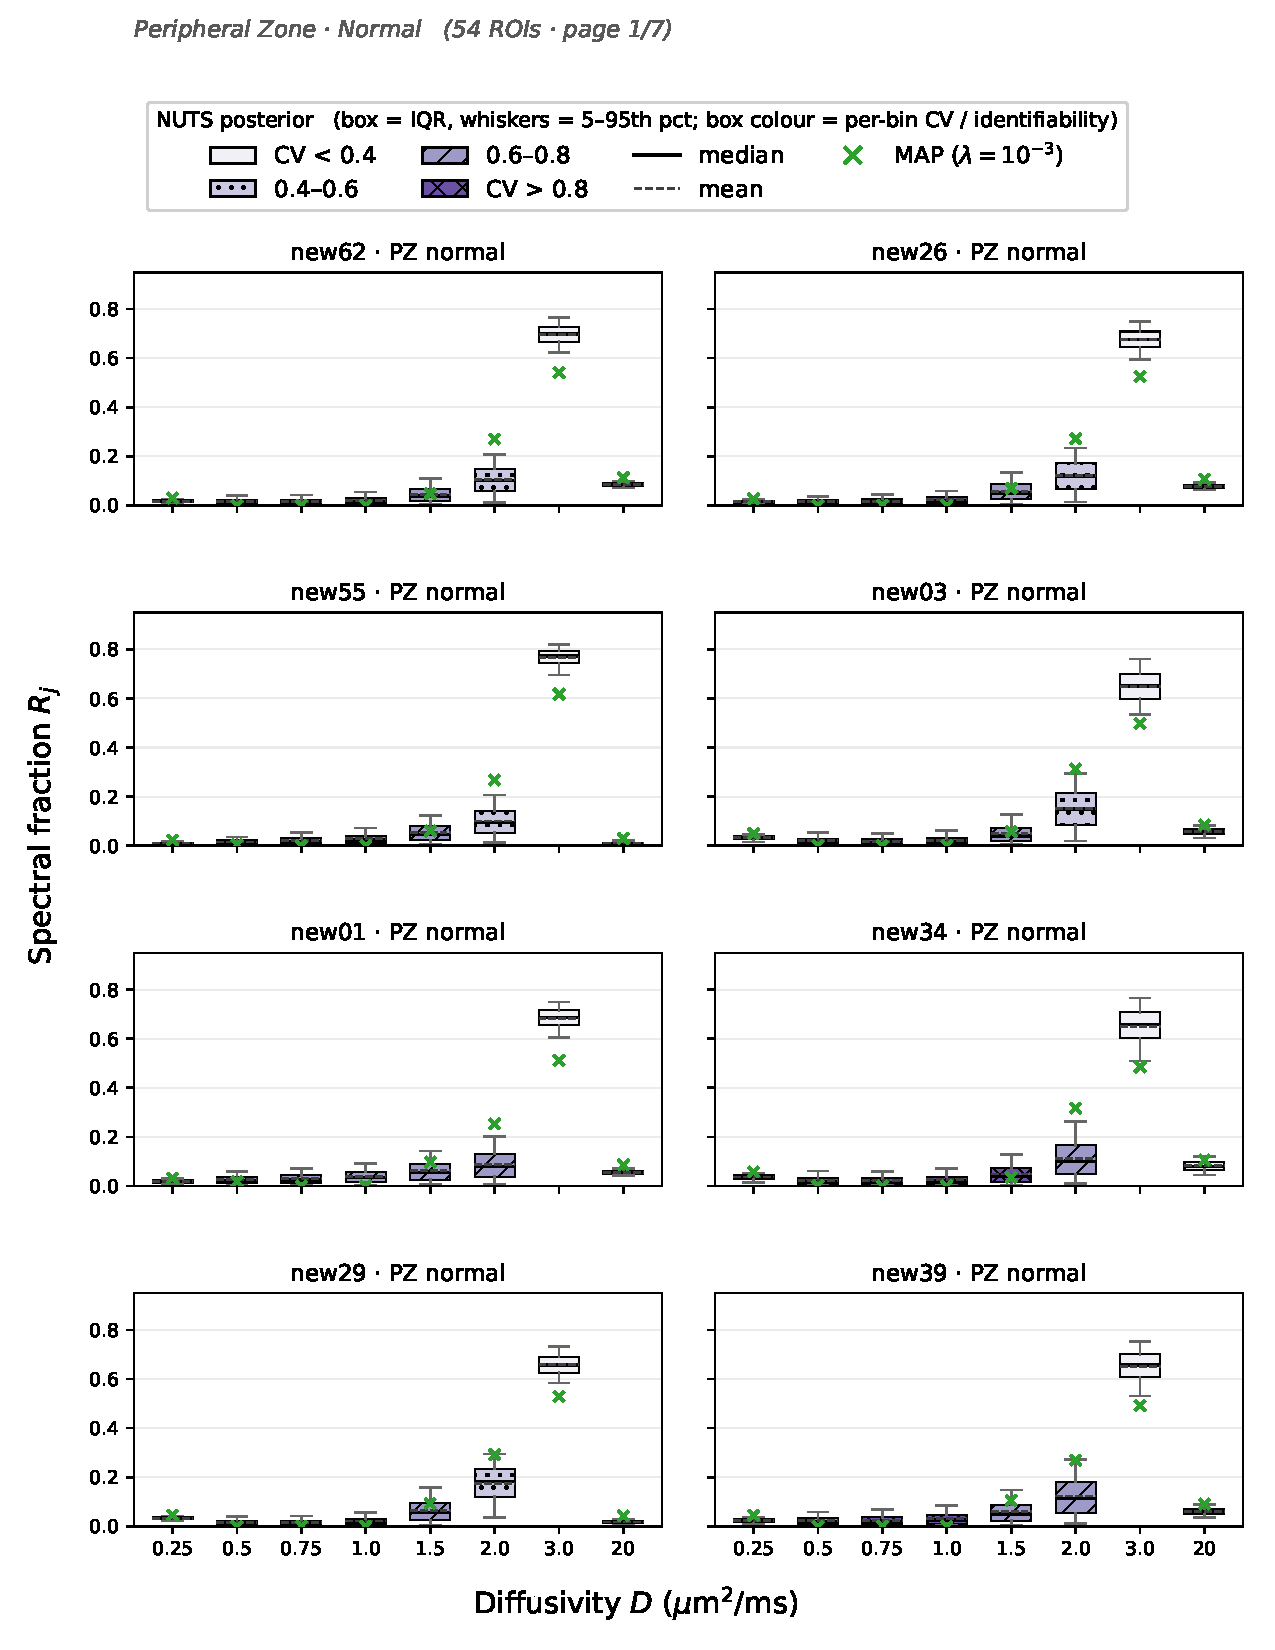
\includepdf[pages=-]{figures/figS1_all_roi_spectra.pdf}

% --- REMOVED 2026-06-02 ---
% Fig S1 (NUTS multi-chain trace plots, fig_trace_simulation.pdf): dropped --
% unreadable and uninformative to readers; convergence is reported in Methods
% (split-Rhat < 1.05 for all 149 ROIs).
% Fig S2 (robustness across spectral shapes, fig_robustness.png): dropped --
% redundant with the recovery panels of main Figure~\ref{fig:validation}, and
% carried unresolved font/colour TODOs. A broader simulation recovery battery
% can be added back to the SI later if desired.

% --- Fig S: Fisher Information Analysis (relocated from the main text 2026-06-01;
%     keeps \label{fig:fisher} so the in-text references in theory/results/discussion
%     resolve to this supplementary figure). ---
\begin{figure}[p]
\centering
% TODO(figure-regen): larger fonts (~+50%); in panel (b) move the legend to
% a free area in the middle of the plot so that it does not cover the bars
% or the improvement-factor labels. NOTE: panel (b) SNR is hard-coded at 150;
% should be regenerated at the cohort-median SNR=303 (see PROJECT_STATE F10).
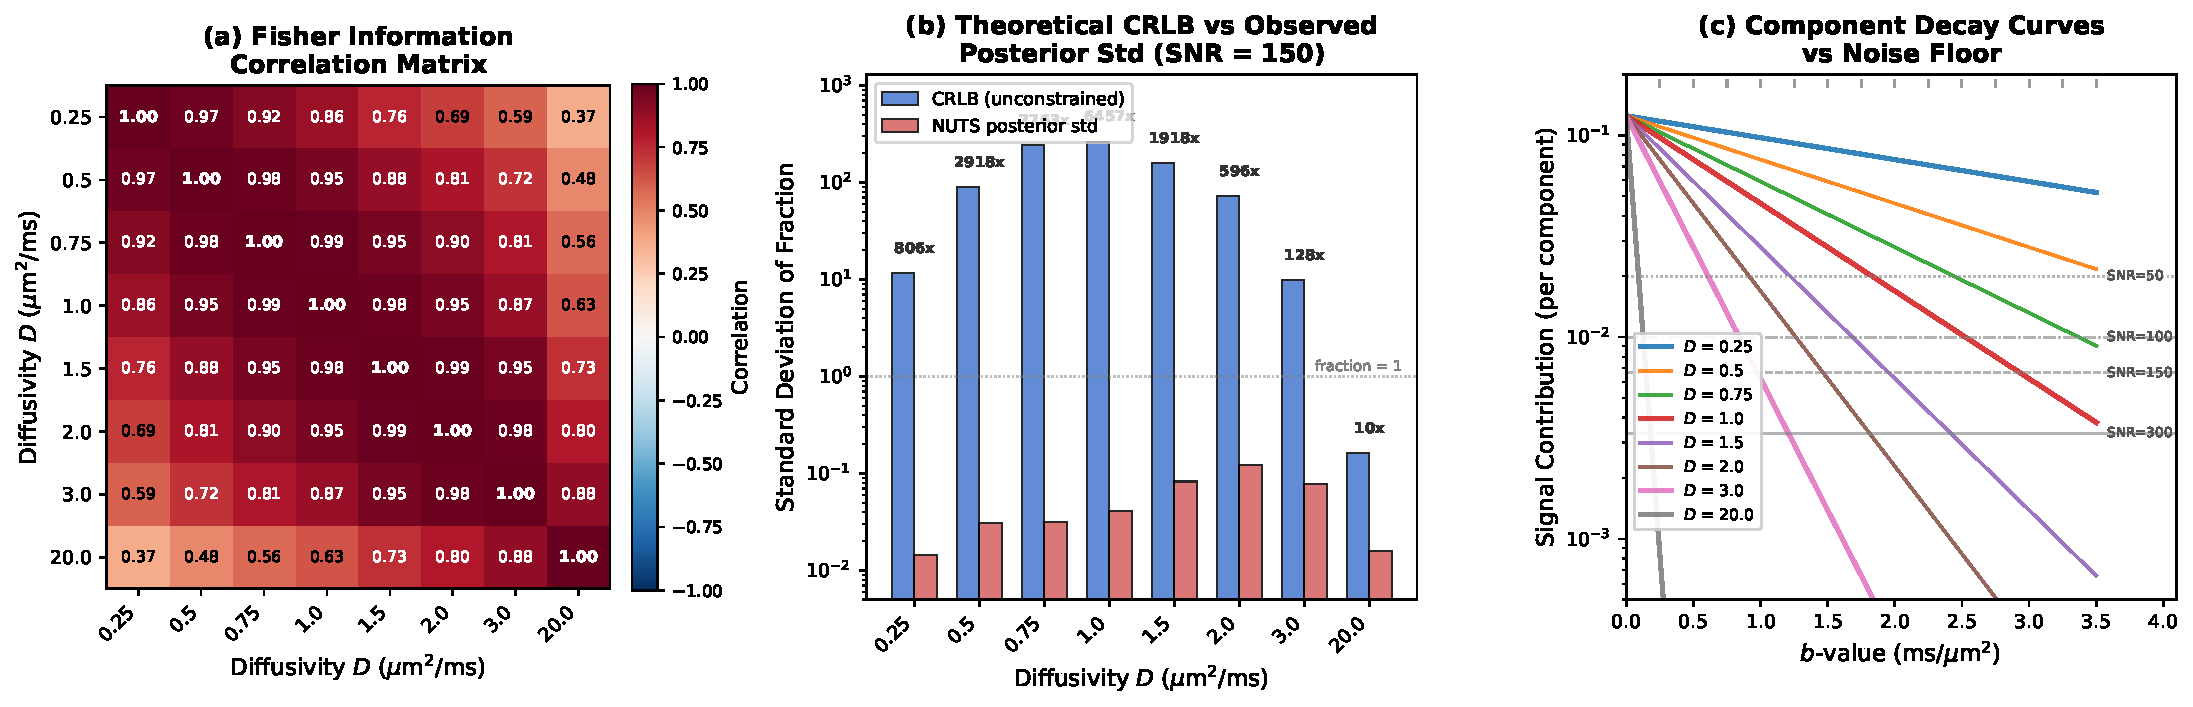
\includegraphics[width=\textwidth]{figures/fig_fisher.pdf}
\caption{%
Fisher information analysis of the spectral discretization.
(a)~Fisher information correlation matrix: adjacent diffusivity components
($D = 0.50$--$1.00\;\umsmm$) have mutual correlation $> 0.99$, making them
fundamentally indistinguishable from 15 b-value measurements.
$D = 0.25$ and $D = 20.0\;\umsmm$ are the most separable components.
(b)~Unconstrained Cram\'er-Rao lower bound (gray) versus observed NUTS
posterior standard deviation (orange) at SNR = 150.
Labels show the improvement factor.
Non-negativity constraints and Bayesian priors reduce estimation error by
100--8000$\times$, demonstrating their essential role.
(c)~Individual component decay curves $R_j \exp(-b D_j) / K$ at equal
fractions, with horizontal noise floors at SNR = 50--300.
Slow-diffusing components (e.g., $D = 0.25\;\umsmm$) contribute signal
across all b-values; fast components ($D \geq 3.0\;\umsmm$) decay below the
noise floor within the first few b-value steps, motivating the sparser
discretization at high diffusivities.
}
\label{fig:fisher}
\end{figure}

%TC:endignore

\end{document}
